\chapter{主板及扩展板PCB设计}
\label{cha:PCB}

主板PCB设计如图~\ref{fig:CorePCB}:

\begin{figure}[htbp]
    \centering
    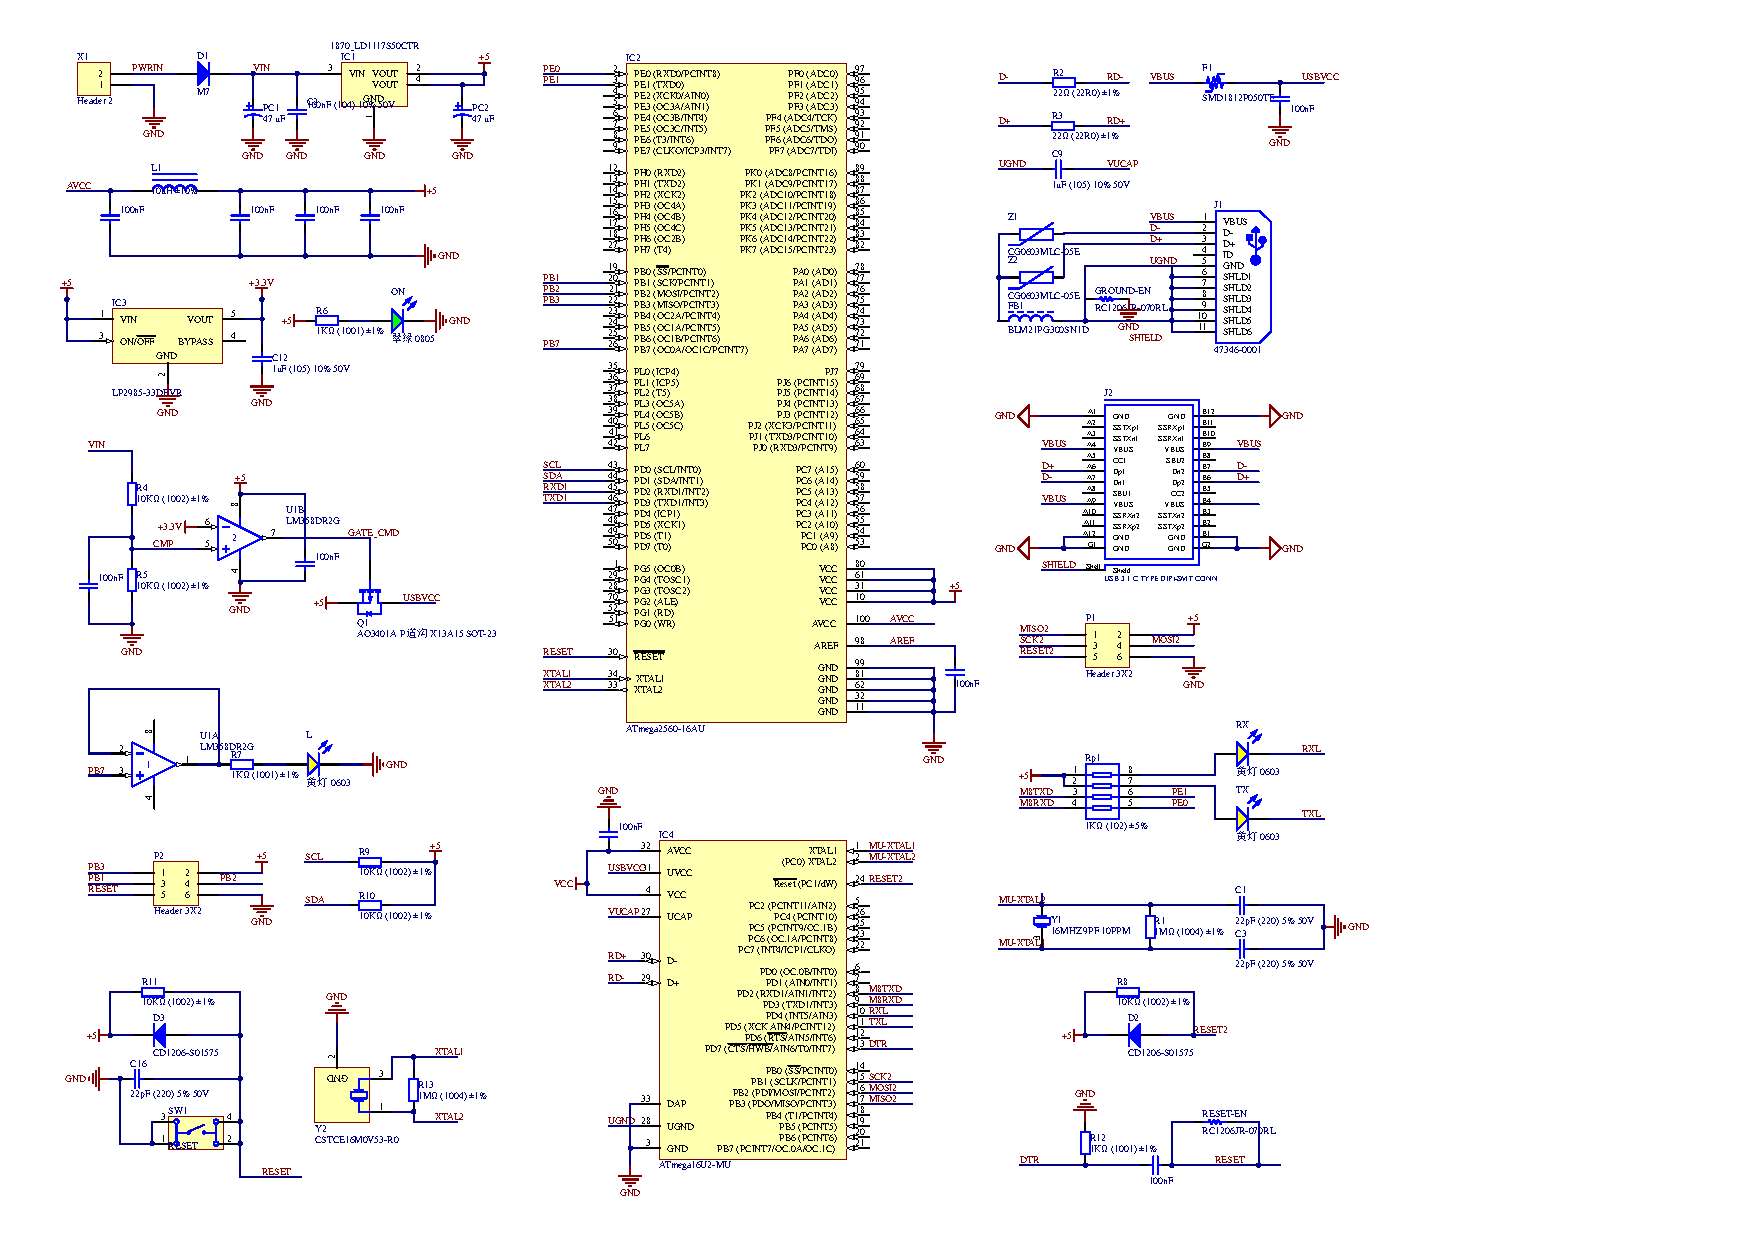
\includegraphics[width=\columnwidth]{ArduinoMega2560-Core-White-Crop.pdf}
    \caption{Mega 2560主板设计}
    \label{fig:CorePCB}
\end{figure}

\section{主控ATmega2560-16AU}

主控芯片采用ARDUINO MEGA 2560 REV3\cite{arduino_mega-2560-r3}上使用的ATmega2560-16U芯片\footnote{\href{http://www.atmel.com/Images/Atmel-2549-8-bit-AVR-Microcontroller-ATmega640-1280-1281-2560-2561_datasheet.pdf}{ATmega2560 Datasheet}},并参考MEGA 2560的芯片外设和烧写器设计。引脚映射图见附录~\ref{sec:Pin2560}。

\begin{figure}[htbp]
    \centering
    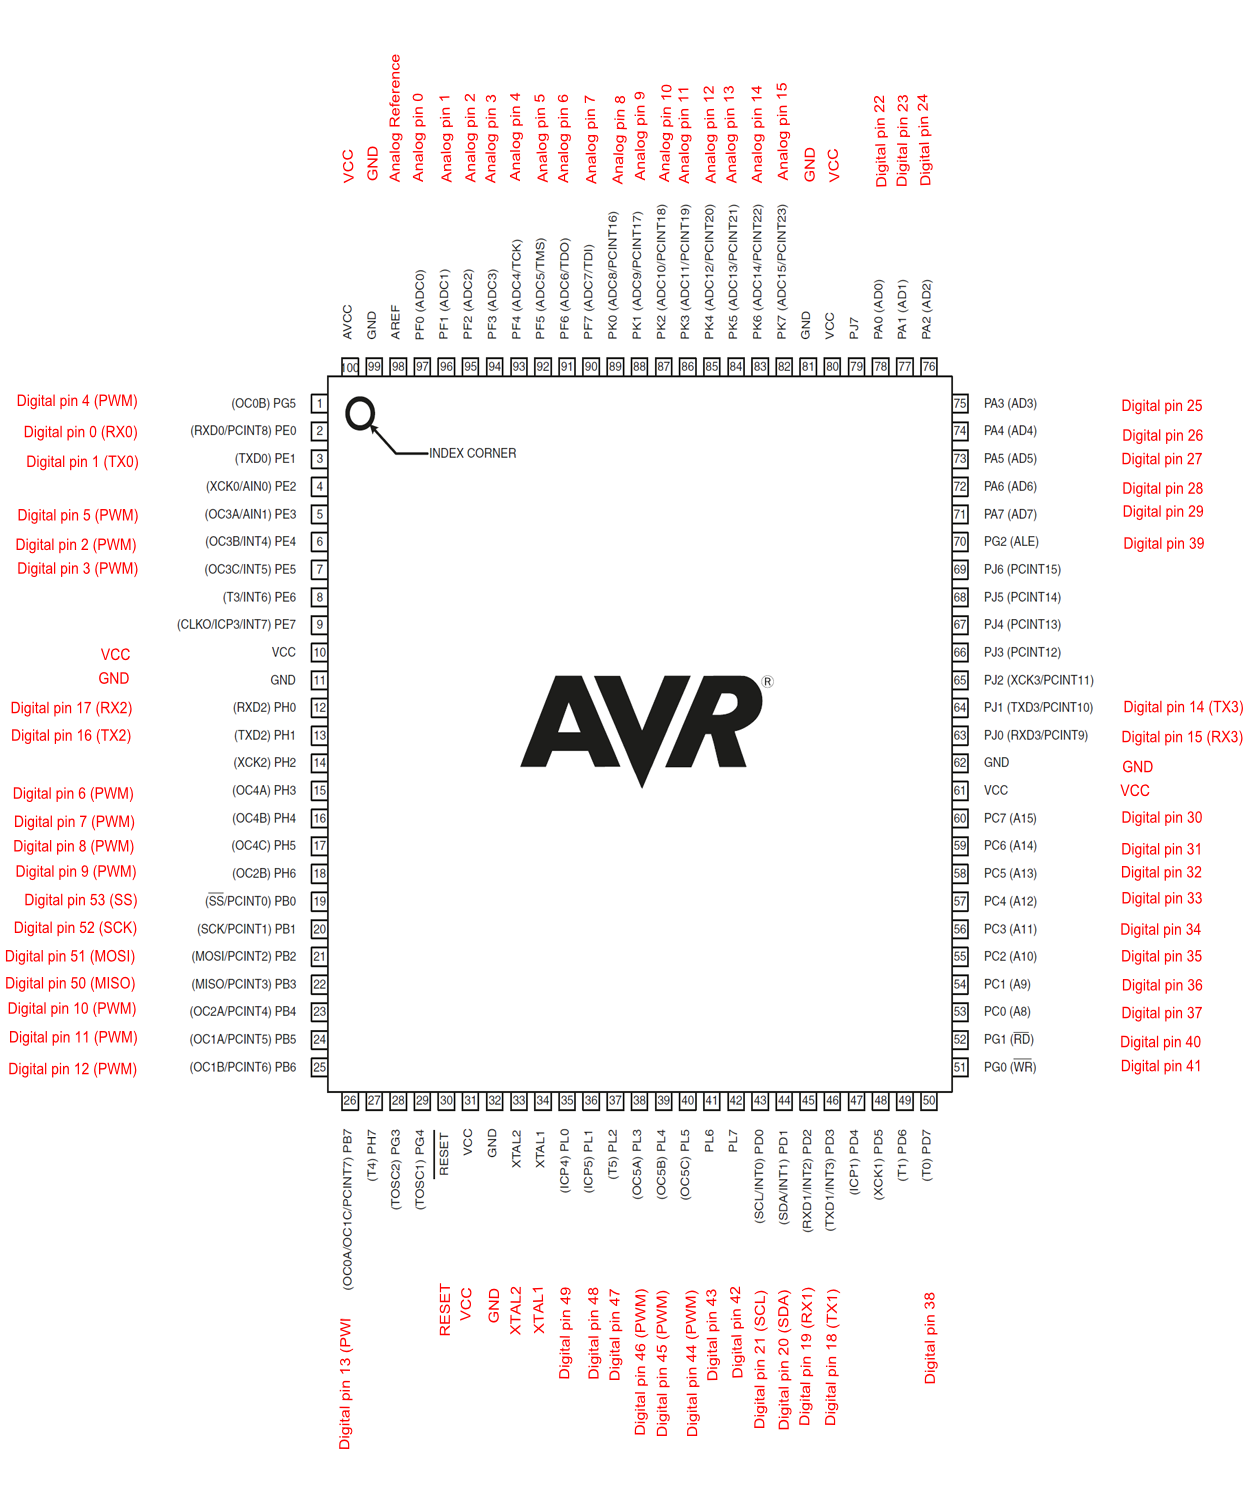
\includegraphics[width=0.7\textwidth]{PinMap2560big_Rev2.png}
    \caption{Mega 2560 PIN diagram}
    \label{fig:PinMap2560}
\end{figure}

ATmega2560是高性能,低功耗基于Microchip 8位AVR RISC的微控制器(MCU),256KB ISP闪存,8KB SRAM,4KB EEPROM,86个GPIO,32个通用工作寄存器,实时计数器,六个具有比较模式的灵活定时器/计数器,PWM,4个USART,面向字节的2线串行接口,16通道10位A/D转换器以及用于片上调试的JTAG接口。该器件在16 MHz时可达到16 MIPS的吞吐量,并在4.5至5.5伏之间工作。通过在单个时钟周期内执行指令,该设备可实现接近1MIPS/MHz的吞吐量,从而平衡了功耗和处理速度。

\begin{figure}[htbp]
    \centering
    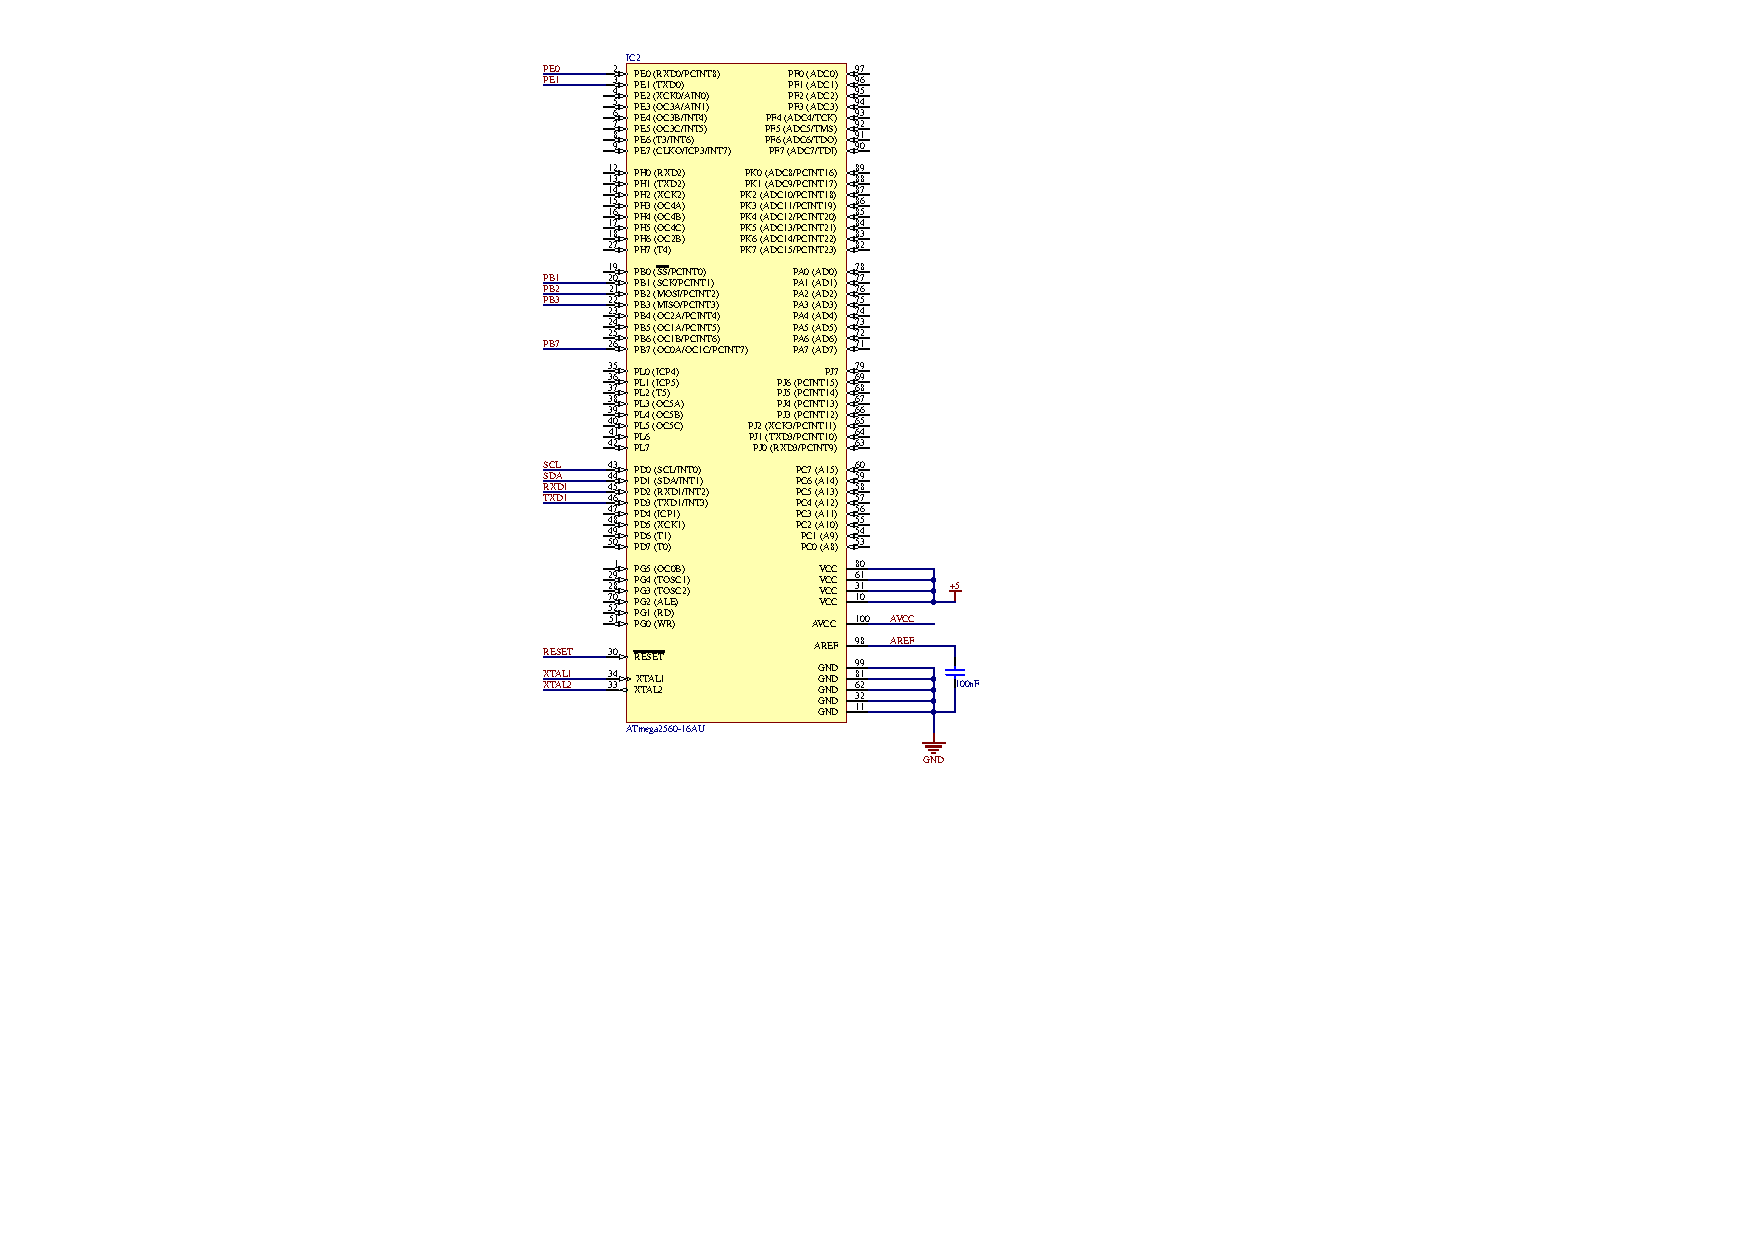
\includegraphics[]{Mega2560-ATmega2560-16AU.pdf}
    \caption{Mega 2560 MCU 原理图}
    \label{fig:Mega2560-ATmega2560-16AU}
\end{figure}

\section{供电和稳压电路}

\begin{figure}[htbp]
    \centering
    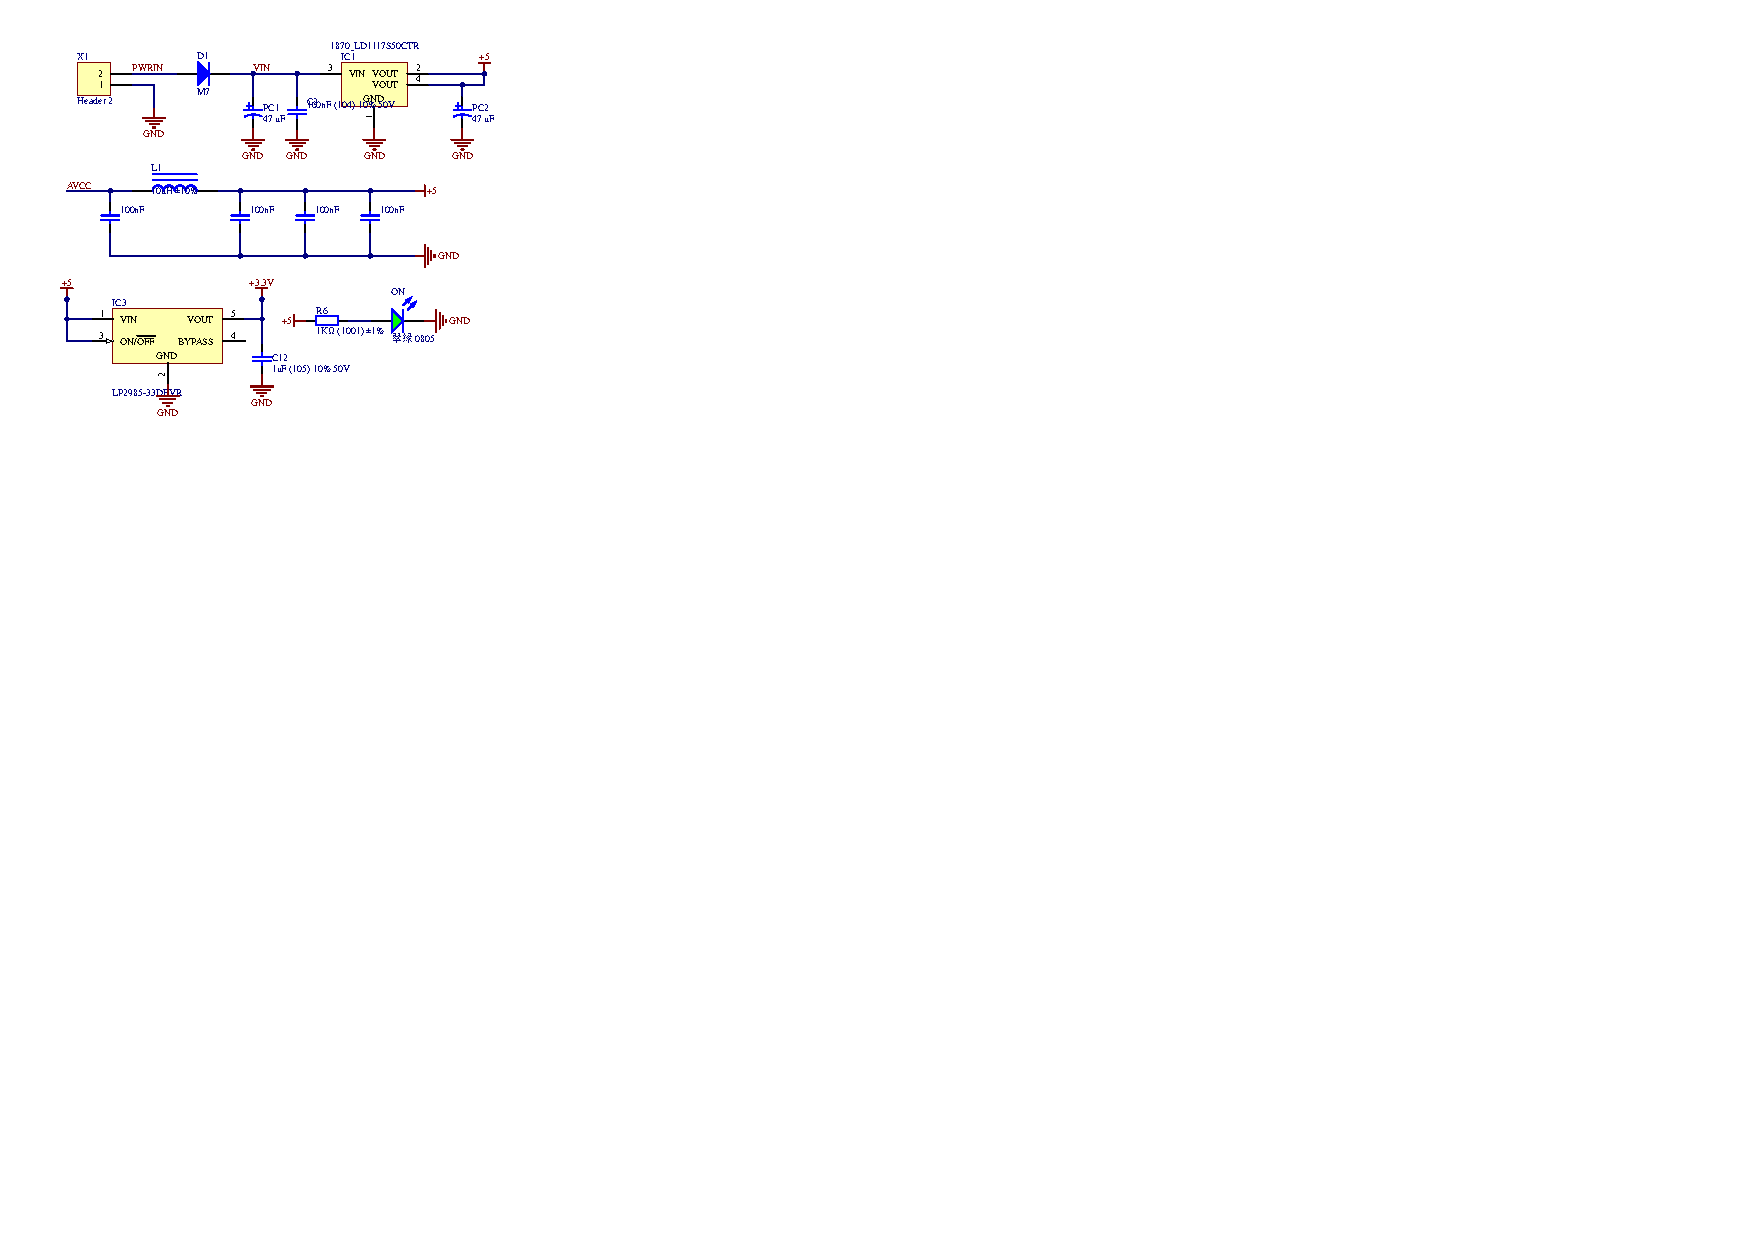
\includegraphics[]{Mega2560-Power.pdf}
    \caption{供电和稳压电路}
    \label{fig:Mega2560-Power}
\end{figure}

如图~\ref{fig:Mega2560-Power},外部锂电通过PWRIN接口输入7-15v直流,两级滤波,使用小电容100nF滤除高频干扰,大电容47uF消除低频干扰,M7为二极管,防止错误输入负电压。低压差线性稳压(LDO)降压芯片LD1117S50CTR完成电平转换,输出5V直流,在输出端也加入了一个47uF的滤波电容,滤除输出5V中的低频谐波。

高通滤波电容原本建议方案使用47uF 35V贴片型铝电解电容器,但是考虑到后续可能要堆叠电路板模块,需要尽可能的减小电路板上元件的最大高度,而6.3x5.4x5.4mm SMD 封装高度达到5.4mm。

可以用CASE-E-7343封装47uF 35V钽电容\footnote{钽电容全称是钽电解电容,也属于电解电容的一种,使用金属钽做电介质}。多数情况下,在不考虑容量和耐压时钽电解可以替换铝电解,但在耐受瞬态尖峰过压和瞬态大电流放电方面,钽电解不及铝电解,某些场合下的一些变通用法,会使电容两端施加小幅反向电压,钽电解也不可以这样。

固体钽电容器电性能优良,工作温度范围宽,而且形式多样,体积效率优异,具有其独特的特征:钽电容器的工作介质是在钽金属表面生成的一层极薄的五氧化二钽膜。此层氧化膜介质与组成电容器的一端极结合成一个整体,不能单独存在。因此单位体积内所具有的电容量特别大。即比容量非常高,因此特别适宜于小型化。但是钽电容

钽电容具有较大的ESR(串连等效电阻)值,瞬态大电流放电特性因而不佳,用于电源的主滤波是不行的,但其串连等效电感低于常见卷绕而成的铝电解,故高频滤波特性比铝电解好,适用于对付高频分量的辅助滤波。

AVCC是端口F和A/D转换器的电源电压引脚。即使不使用ADC,它也应从外部连接到VCC。如果使用ADC,则应通过低通滤波器将其连接到VCC。

LP2985-33DBVR则是另一个低压差线性稳压(LDO),它将5V降到3.3V。根据Datasheet,在布线时,旁路电容器的放置应尽可能的接近器件的VIN和系统的GND,注意使旁路电容器连接VIN引脚和系统的GND引脚形成的环路面积最小。

绿色LED串联1KOhm保护电阻,当电路接上电源时,ON LED将发光作为提示。

\begin{figure}[htbp]
    \centering
    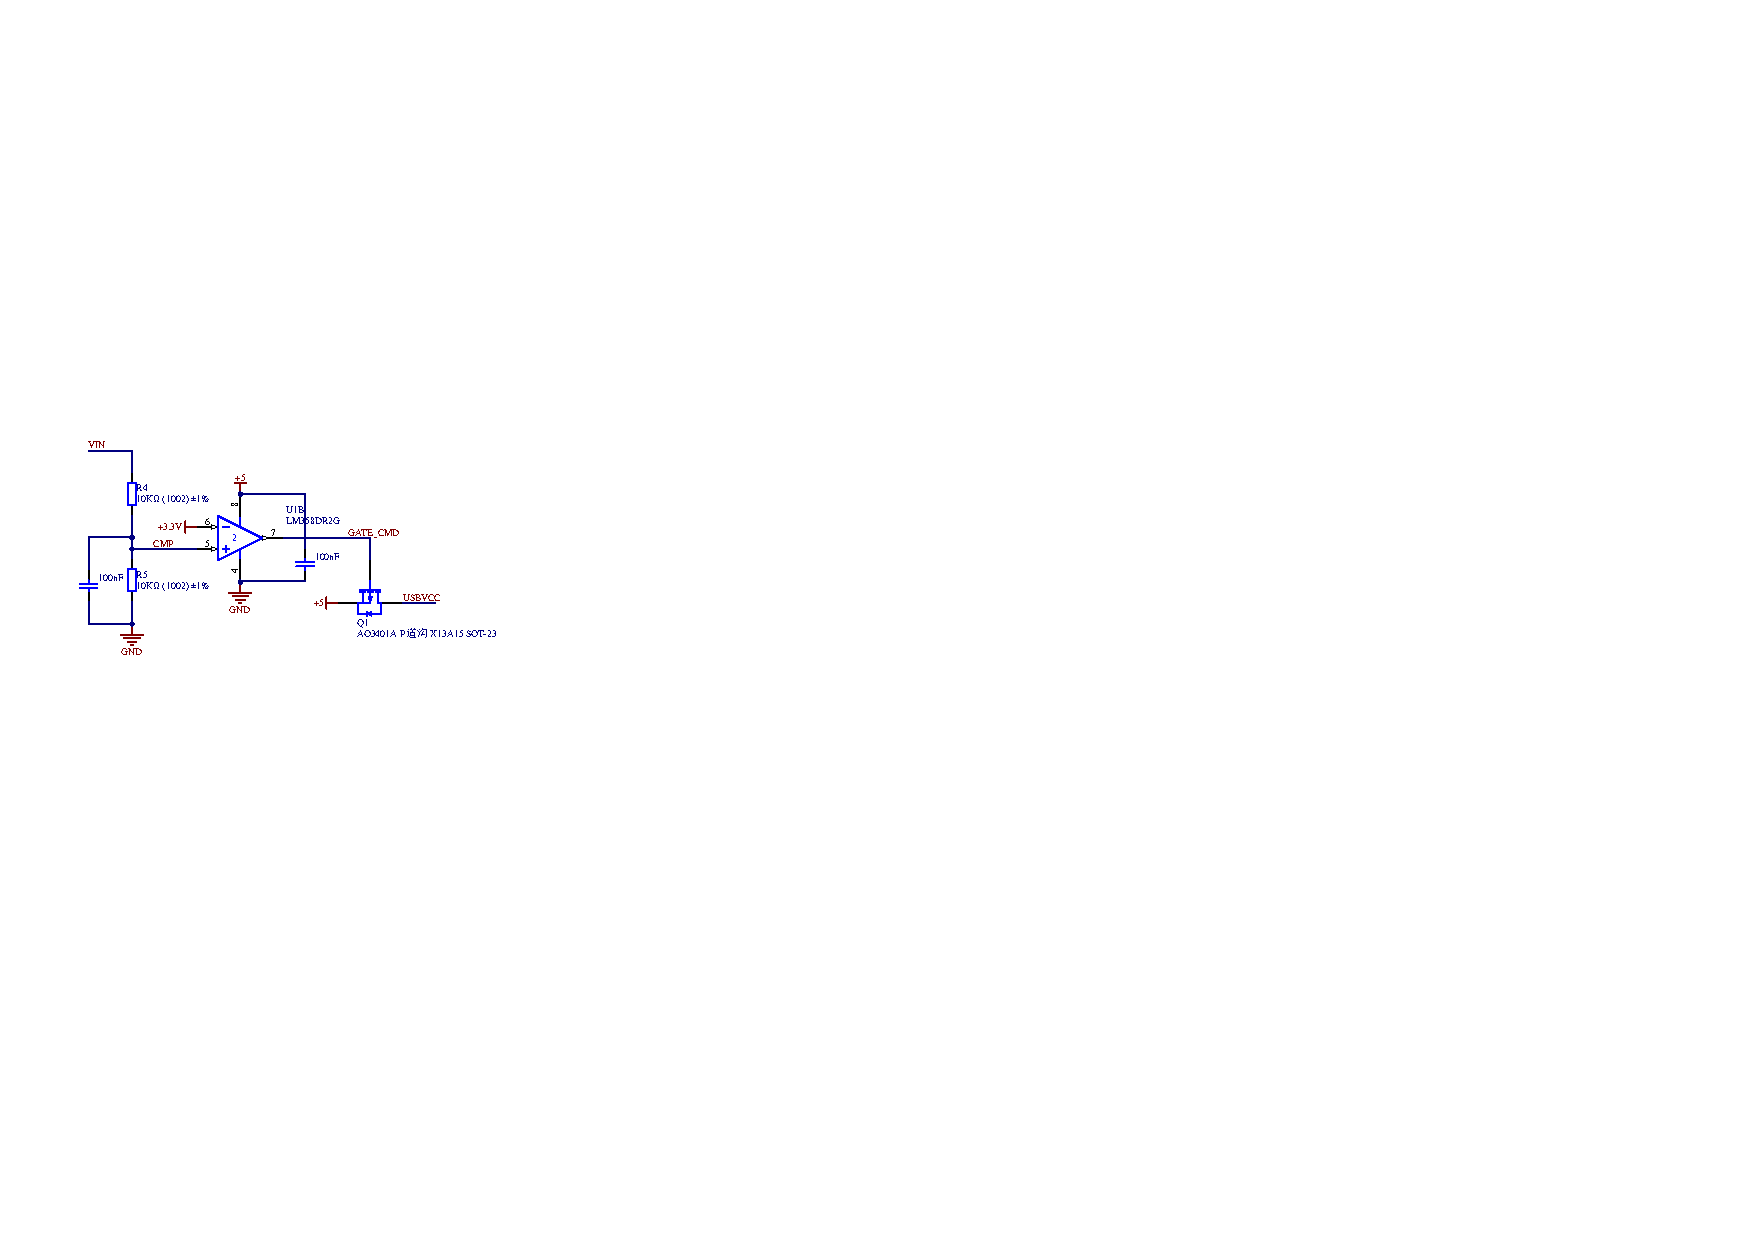
\includegraphics[]{Mega2560-USB-POWER.pdf}
    \caption{USB供电选择电路}
    \label{fig:Mega2560-USB-POWER}
\end{figure}

如图~\ref{fig:Mega2560-USB-POWER},LM358DR2G为增益带宽积(GBP)1MHz的通用双路运放,AO3401A则为P沟道MOS(场效应管),低电平导通。

LM358DR2G的B路运放在这里作为电压比较器使用,若VIN大于6.6V,即有锂电输入,此时运放输出高电平,PMOS关断,此时板上供电由锂电提供,同时也切断了USB,防止通过锂电给USB供电的情况出现。当VIN没有输入,即没有锂电输入,如果此时USB接通,PMOS导通,USB可以直接给板子供应5V直流。

\section{MCU附属IO}

\begin{figure}[htbp]
    \centering
    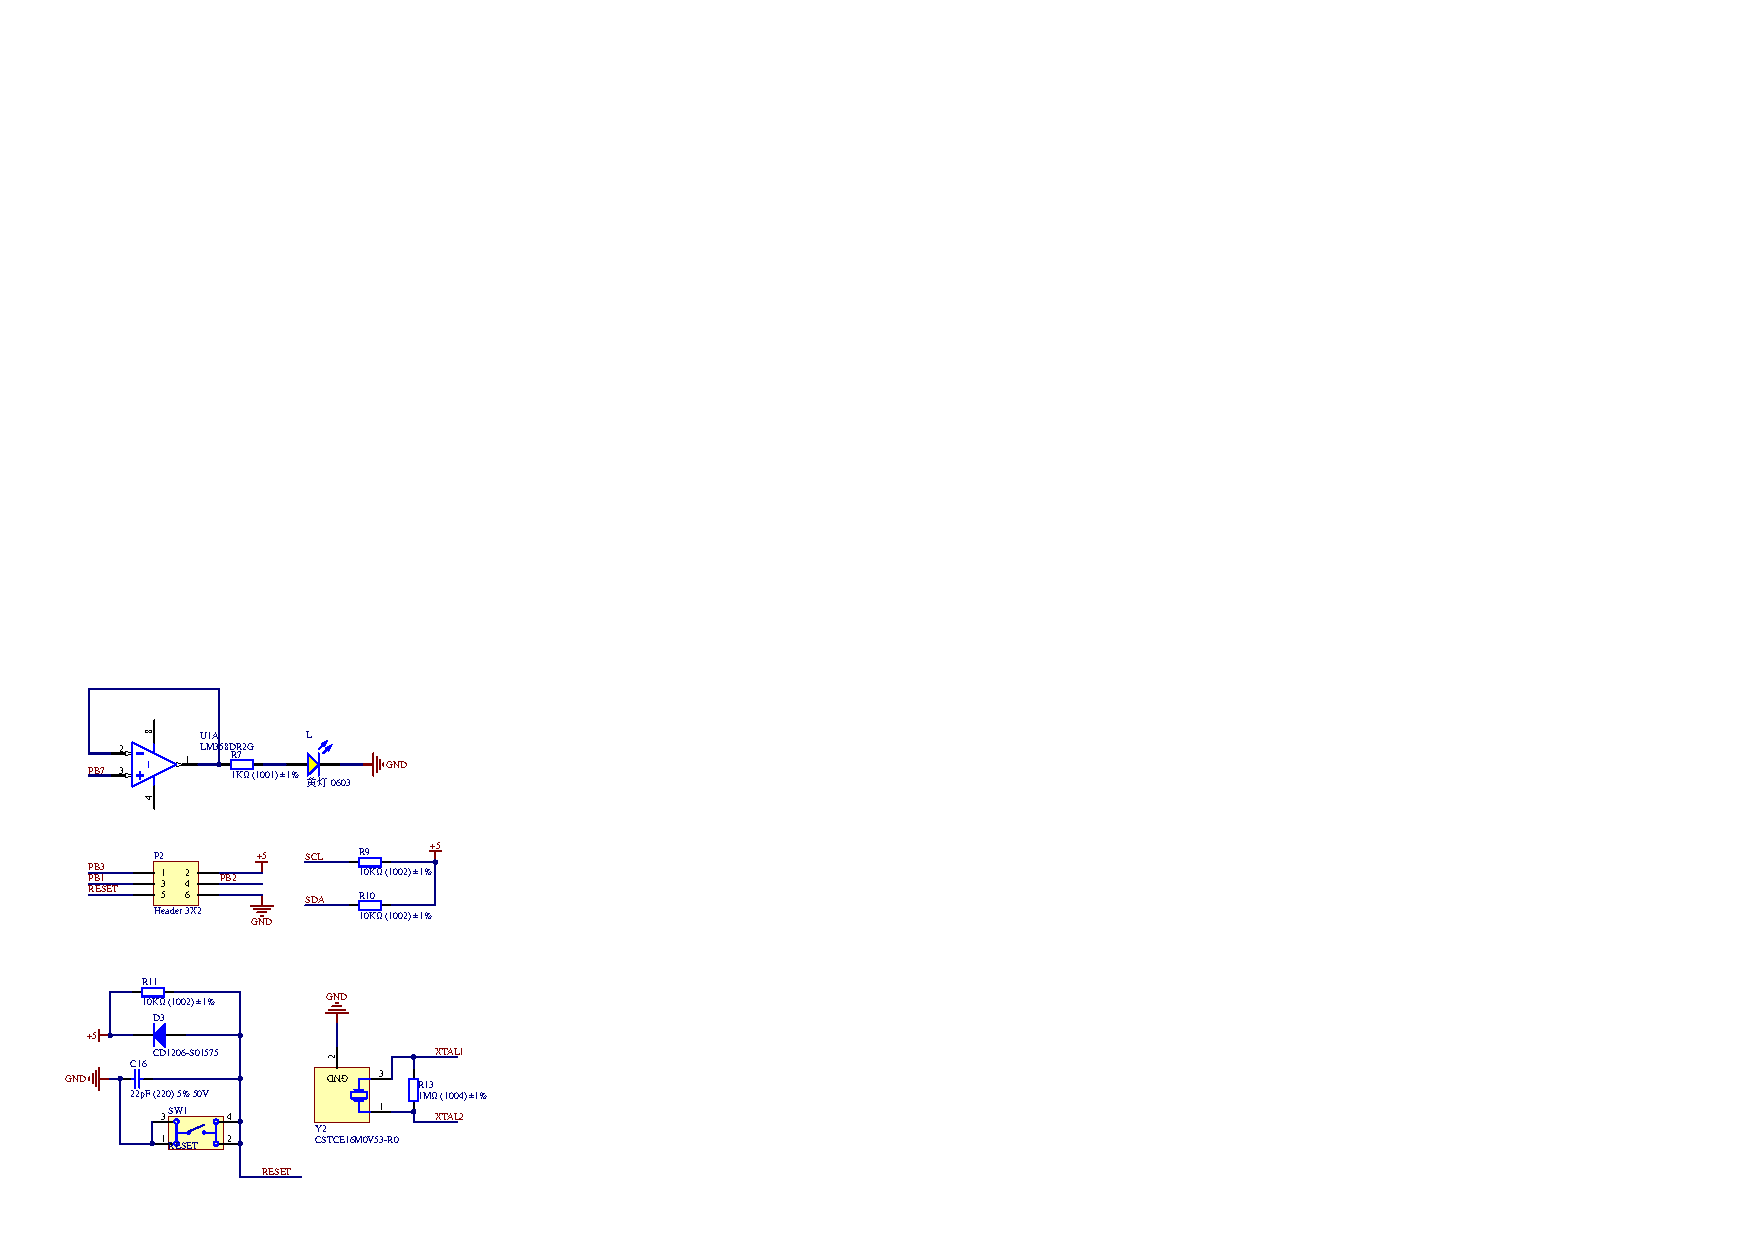
\includegraphics[]{Mega2560-Core-IO.pdf}
    \caption{MCU附属IO}
    \label{fig:Mega2560-Core-IO}
\end{figure}

如图~\ref{fig:Mega2560-Core-IO},LM358DR2G的A路运放在这里作为电压跟随器,作为黄色LED的驱动,接收PB7即D13引脚的数字输入,控制黄色LED的亮灭。

2x3的端子是ICSP (In-Circuit Serial Programming) 端口,可以通过这个6Pin端口给ATmega2560 MCU烧写程序。结合AVR-ISP (in-system programmer)比如Arduino ISP\footnote{https://store.arduino.cc/usa/arduino-isp}使用。

使用Arduino ISP,可以上传脚本并在任何基于AVR的板上烧写引导程序。通过使用外部编程器上传Sketch,可以删除引导程序bootloader。Arduino ISP还可用于刻录Arduino bootloader,因此,如果不小心损坏了bootloader,则可以用它来恢复。当使用新的ATmega MCU时,也有必要刷引导程序,将希望使用的引导程序通过USB-Serial连接上传。

SCL和SDA为I2C(Inter-Integrated Circuit)集成电路总线,是一种串行通讯汇流排,使用多主从架构,只使用两条双向漏极开路(Open Drain)(串行资料(SDA)及串行时脉(SCL))并利用电阻将电位上拉。这里两个10kOhm电阻即为I2C上拉电阻。

按下轻触开关,MCU的RESET从高电平变为低电平,MCU中的程序复位,相当于重启。

CSTCE16M0V53为16MHz晶振,内置电容,作为MCU的外部时钟晶振使用。

\section{ATmega16U2}

\begin{figure}[htbp]
    \centering
    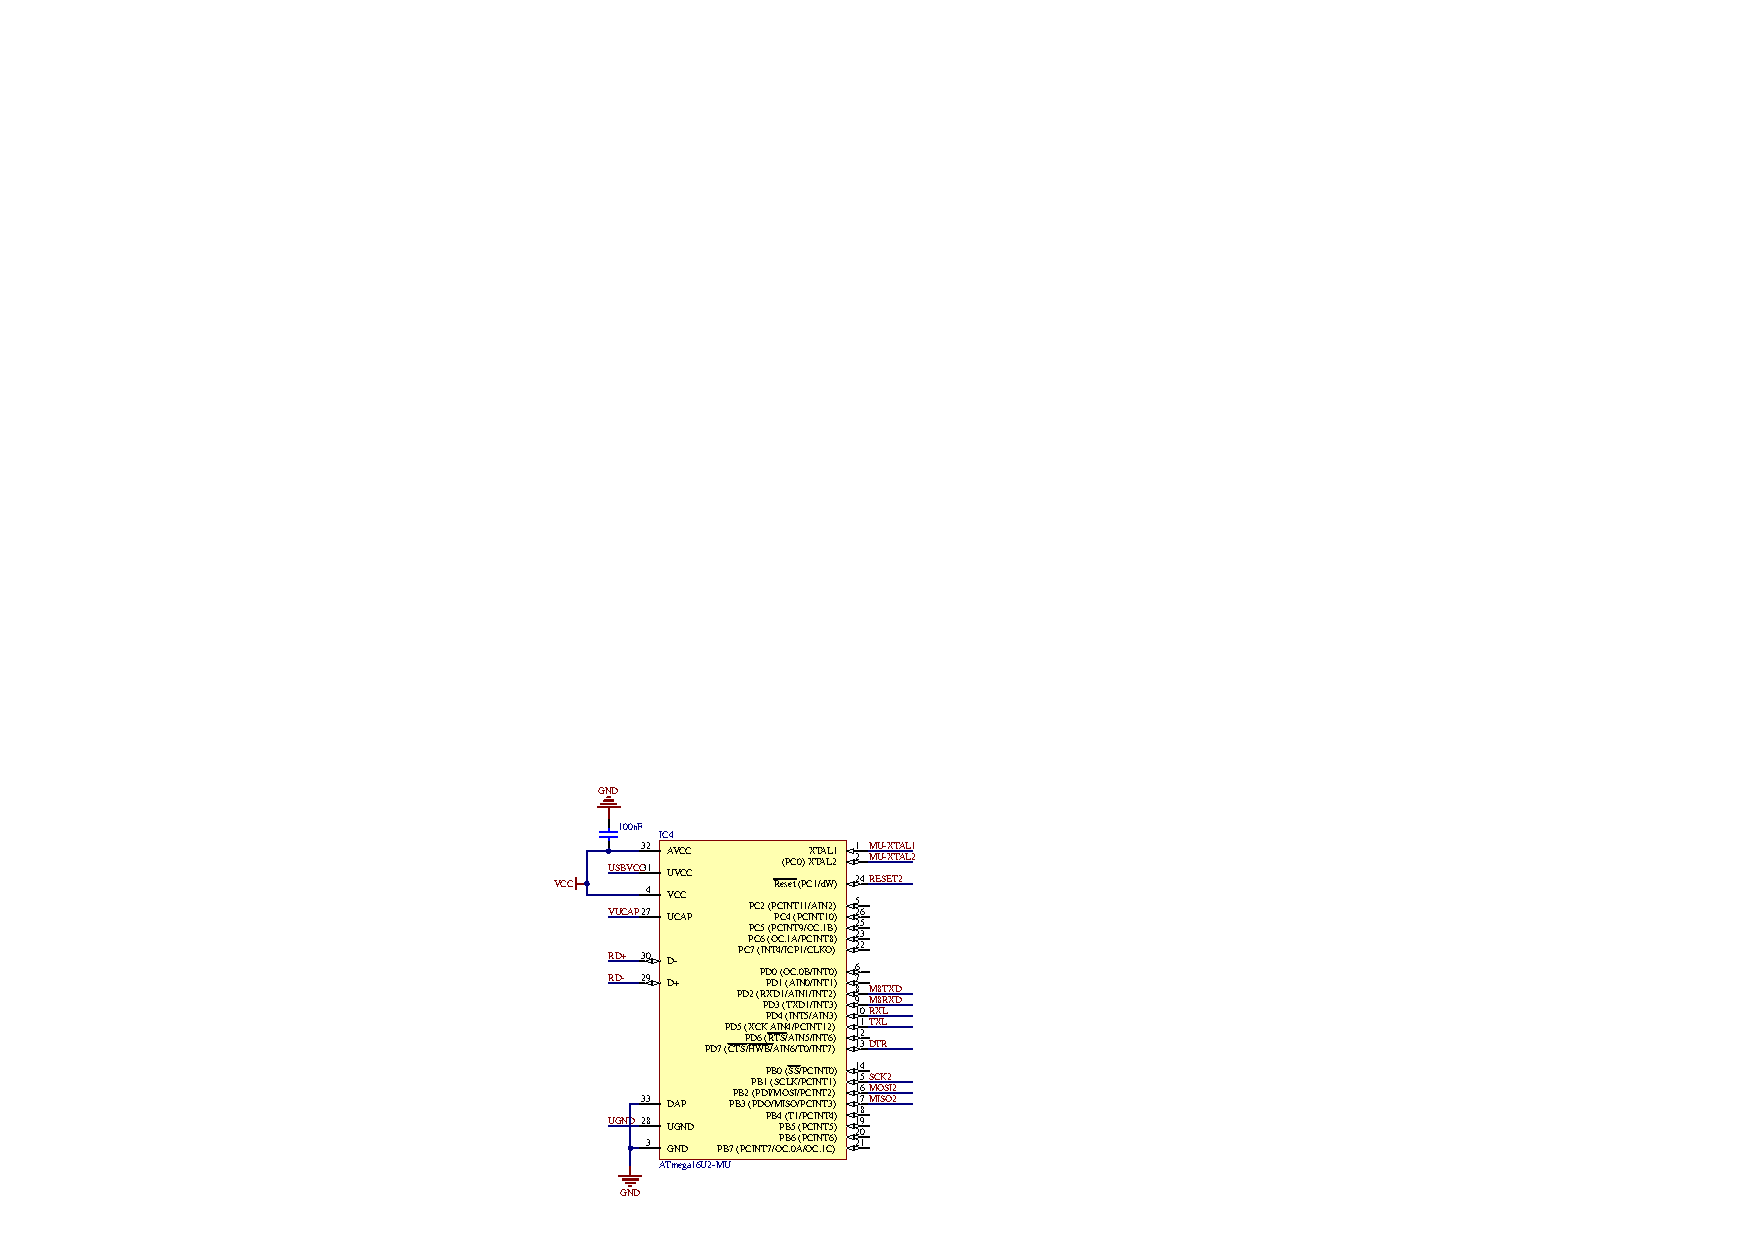
\includegraphics[]{Mega2560-ATmega16U2-MU.pdf}
    \caption{Mega2560-ATmega16U2-MU}
    \label{fig:Mega2560-ATmega16U2-MU}
\end{figure}

如图~\ref{fig:Mega2560-ATmega16U2-MU},板上的ATmega16U2芯片充当计算机的USB端口和主处理器ATmega2560-16AU的串行端口之间的桥梁。它运行称为固件的软件(之所以这样命名,是因为一旦在芯片中对其进行编程就无法更改),该软件可以通过称为DFU(设备固件更新)的特殊USB协议\footnote{https://www.arduino.cc/en/Hacking/DFUProgramming8U2}进行更新。

\begin{figure}[htbp]
    \centering
    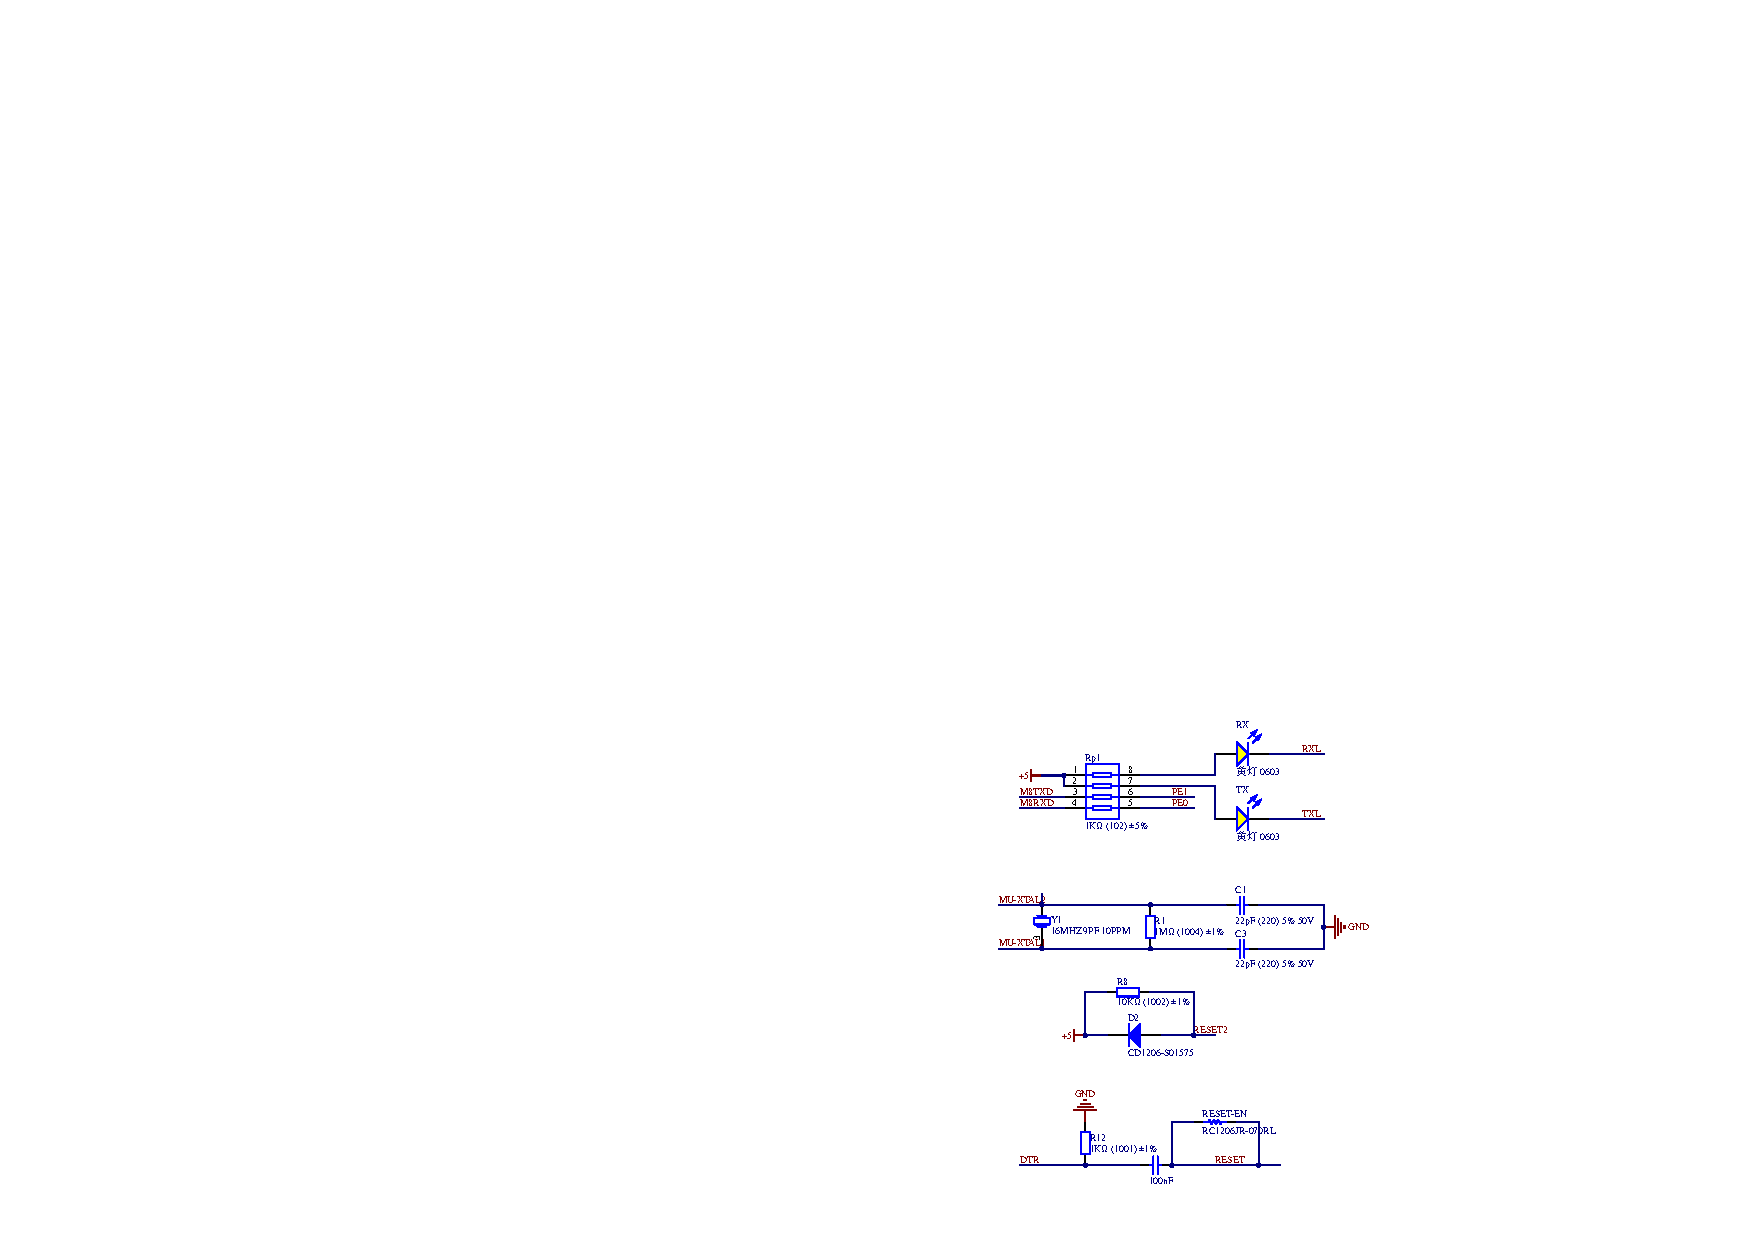
\includegraphics[]{Mega2560-MU-IO.pdf}
    \caption{Mega2560-MU-IO}
    \label{fig:Mega2560-MU-IO}
\end{figure}

如图~\ref{fig:Mega2560-MU-IO}:

2x3的端子是ICSP (In-Circuit Serial Programming) 端口,可以通过这个6Pin端口给ATmega16U2 MCU烧写程序。

Rp1为一个排阻,上有四个相同阻值(1kOhm)的电阻,上面两个电阻作为两个黄灯的保护电阻,两个黄灯作为RX1和TX1数据传输的指示。另两个电阻则是从ATmega16U2到ATmega2560-16AU的通信线路上的电阻,通过ATmega2560-16AU的PE0和PE1给MCU烧写程序。

RESET-EN为自动复位设计,可以通过主机复位。这样通过Arduino软件烧写程序到Mega2560中软件可以自动复位,不需要再按复位按钮。在PCB上切断"RESET EN"处两个焊盘中间的线可以禁止该功能。

\section{USB接口}

通过通用串行总线(英语:U niversal S erial B us,缩写:USB)对MCU进行程序烧写和部分数据交换,同时可以给电路板供电。

USB在速度上远比并行端口(例如EPP、LPT)与串行接口(例如RS-232)等传统电脑用标准汇流排快上许多。USB 2.0(USB 2.0 HiSpeed)为480Mbps,USB 3.0(USB 3.2 Gen1)为5Gbps,USB 3.1(USB 3.2 Gen2x1)为10Gbps,而USB 3.2(USB 3.2 Gen2x2)更达20Gbps。

由于不需要过快的数据交换速度,选用USB 2.0(USB 2.0 HiSpeed)协议进行数据交换。

% https://tex.stackexchange.com/questions/316435/how-to-put-6-images-in-3-columns-2-rows/316444
% 在此环境插入png会报错,得是pdf
% https://tex.stackexchange.com/questions/17734/cannot-determine-size-of-graphic
\begin{figure}[htbp]
    \centering % <-- added
    \begin{subfigure}{0.25\textwidth}
    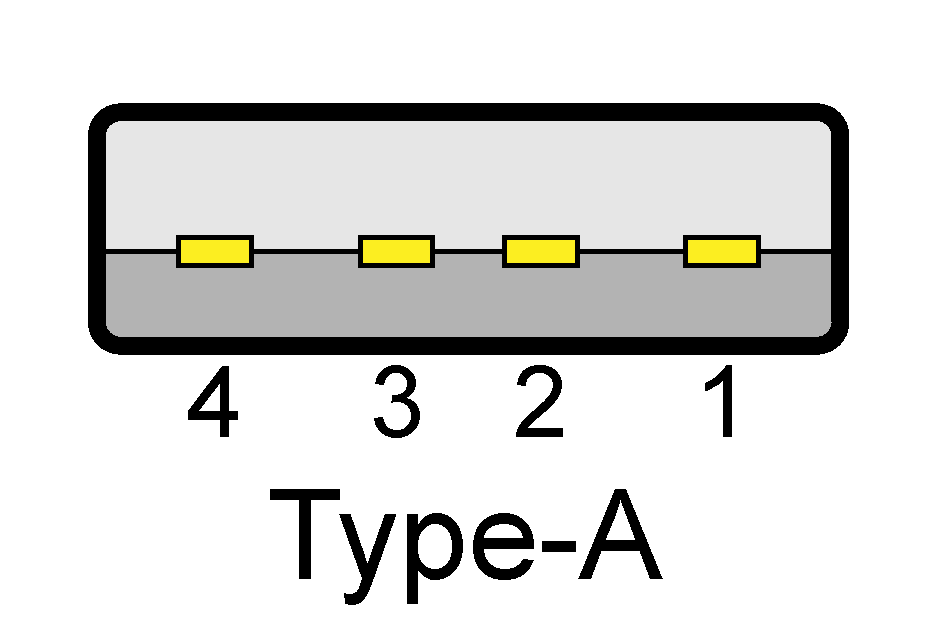
\includegraphics[width=\linewidth]{USB_Type-A.pdf}
    \caption{USB Type-A 公头}
    \label{fig:USB-1}
    \end{subfigure}\hfil % <-- added
    \begin{subfigure}{0.25\textwidth}
    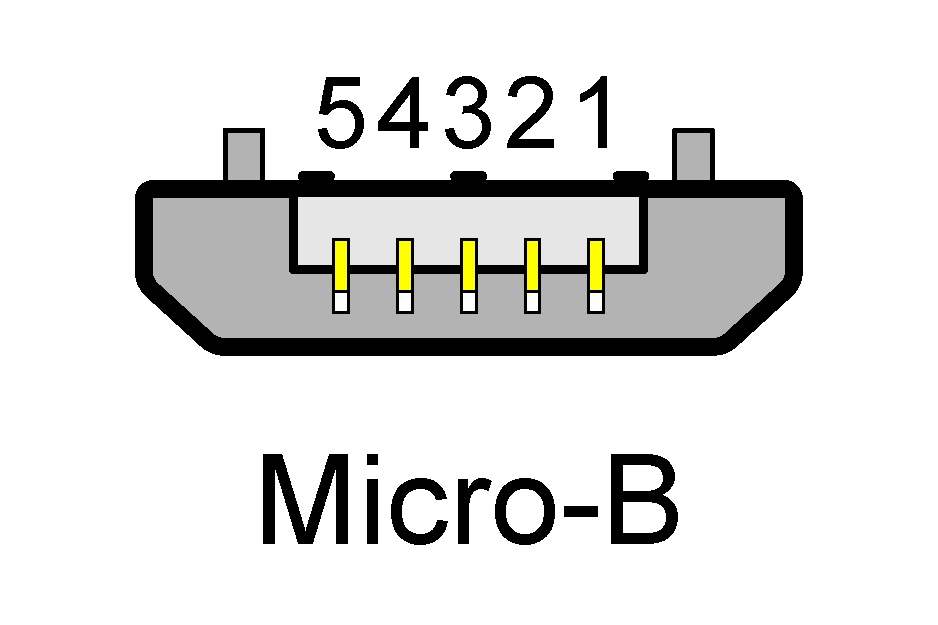
\includegraphics[width=\linewidth]{USB_Micro-B.pdf}
    \caption{USB Micro-B 公头}
    \label{fig:USB-2}
    \end{subfigure}\hfil % <-- added
    \begin{subfigure}{0.25\textwidth}
    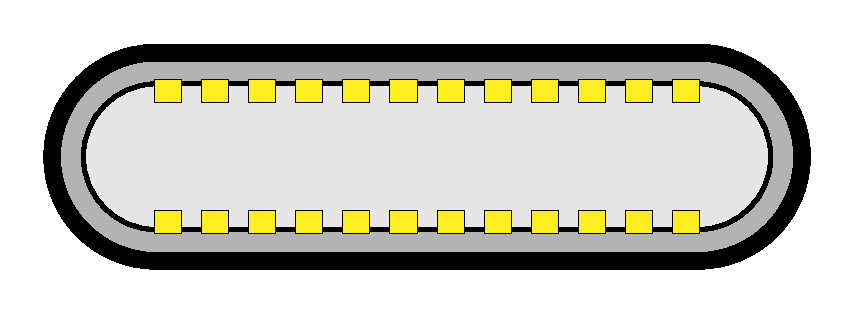
\includegraphics[width=\linewidth]{USB_Type-C_icon.pdf}
    \caption{USB Type-C 公头}
    \label{fig:USB-3}
    \end{subfigure}

    \medskip
    \begin{subfigure}{0.25\textwidth}
    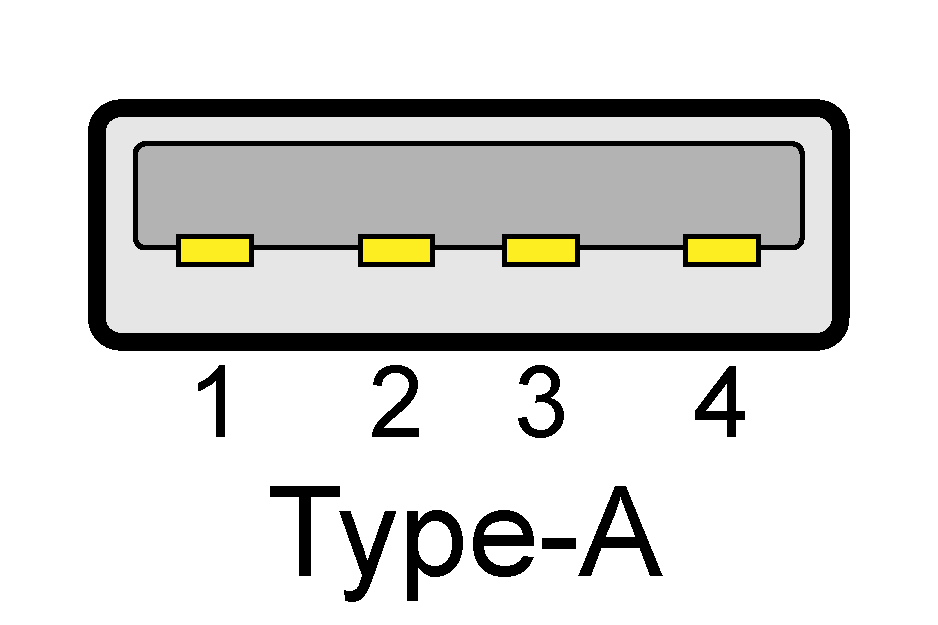
\includegraphics[width=\linewidth]{USB_Type-A_receptacle.pdf}
    \caption{USB Type-A 母头}
    \label{fig:USB-4}
    \end{subfigure}\hfil % <-- added
    \begin{subfigure}{0.25\textwidth}
    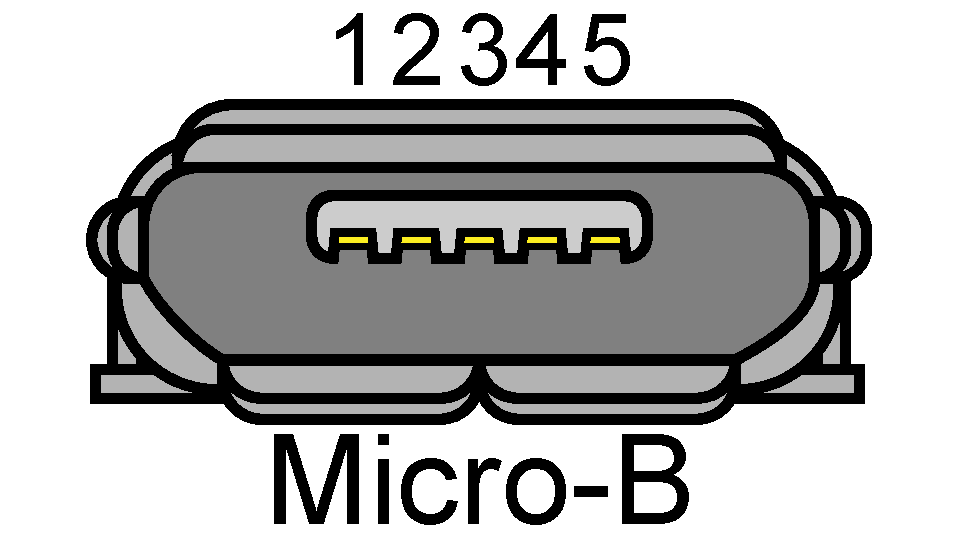
\includegraphics[width=\linewidth]{USB_Micro-B_receptacle.pdf}
    \caption{USB Micro-B 母头}
    \label{fig:USB-5}
    \end{subfigure}\hfil % <-- added
    \begin{subfigure}{0.25\textwidth}
    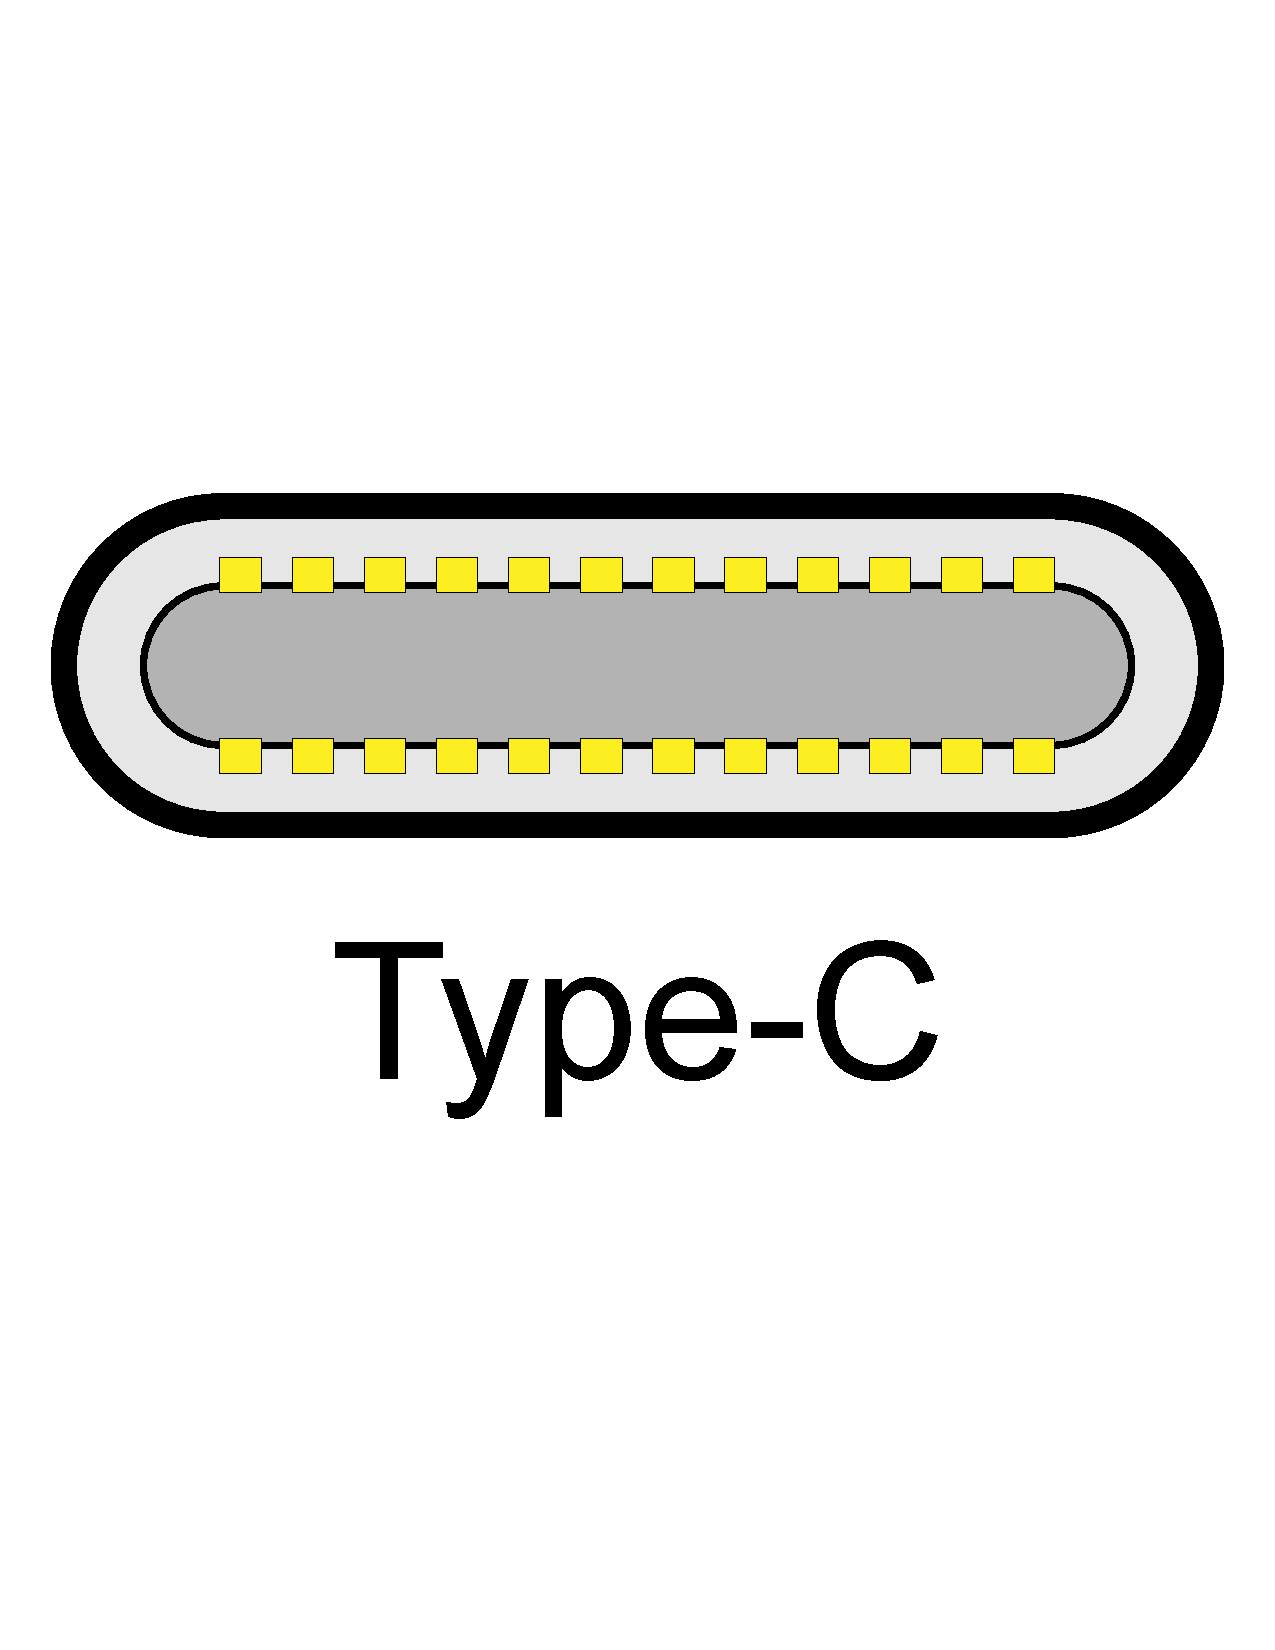
\includegraphics[width=\linewidth]{USB_Type-C_receptacle.pdf}
    \caption{USB Type-C 母头}
    \label{fig:USB-6}
    \end{subfigure}
    \caption{USB 2.0 机械电子标准一览}
    \label{fig:USB-M}
\end{figure}


如表~\ref{fig:USB-M},USB的连接器分为A、B两种,分别用于主机和设备;其各自的小型化的连接器是Mini-A, Mini-B 和 Micro-A, Micro-B,另外还有Mini-AB(可支持Mini-A及Mini-B)的插口。USB 3.1版本中引入了支持正反面不区分插入的C型。

普通电脑上使用的是Type-A口,所以连接电路板时会使用Type-A转Micro USB或Type-C的USB2.0数据线。USB插槽本身还能提供5V的主动电压,及0.5A的电流。

在标准USB接口Type-A中,有四个连接器触点如表~\ref{tab:USB-4},USB信号使用分别标记为D+和D-的双绞线传输,它们各自使用半双工的差分信号并协同工作,以抵消长导线的电磁干扰。

% Please add the following required packages to your document preamble:
% \usepackage{booktabs}
\begin{table}[]
    \centering
    \begin{tabular}{@{}lll@{}}
    \toprule
    触点 & 功能(主机)             & 功能(设备)            \\ \midrule
    1  & V BUS(4.75-5.25 V) & V BUS(4.4-5.25 V) \\
    2  & D-                 & D-                \\
    3  & D+                 & D+                \\
    4  & 接地                 & 接地                \\ \bottomrule
    \end{tabular}
    \caption{标准USB Type-A连接器触点}
    \label{tab:USB-4}
\end{table}

使用Micro-USB机械电子标准的USB插座(母头),此标准常用于移动电话、平板电脑等。Micro-USB将成为移动设备数据和电源的标准接口。

Micro-USB除了第4针外,其他接口功能皆与标准USB相同如表~\ref{tab:MicroUSB}。第4针成为ID,地线在Micro-USB上连接到第5针,在Micro-USB可以悬空亦可连接到第5针。

% Please add the following required packages to your document preamble:
% \usepackage{booktabs}
\begin{table}[]
    \centering
    \begin{tabular}{@{}lll@{}}
    \toprule
    触点 & 功能                & 颜色 \\ \midrule
    1  & V BUS(4.4–5.25 V) & 红  \\
    2  & D−                & 白  \\
    3  & D+                & 绿  \\
    4  & ID                &    \\
    5  & 接地                & 黑 \\ \bottomrule
    \end{tabular}
    \caption{Micro USB连接器触点}
    \label{tab:MicroUSB}
\end{table}

也可以使用支持正反插的USB Type-C接口进行供电和烧写程序,USB Type-C接口常用于新式计算机、移动电话、平板电脑等。其通讯协议和标准见图~\ref{fig:USB-Type-C-pins}和图~\ref{fig:USB-TypeC}。

\begin{figure}[htbp]
    \centering
    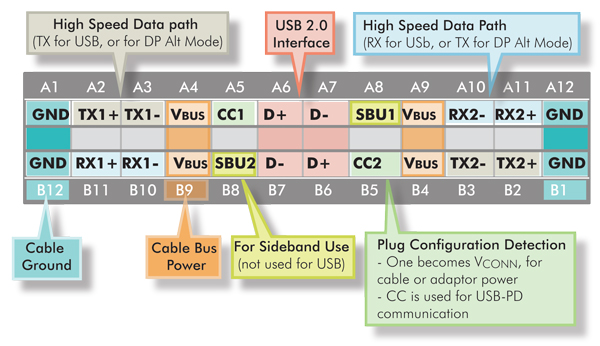
\includegraphics[width=\columnwidth]{Figure-2-USB-Type-C-pins.jpg}
    \caption{USB-Type-C-pins}
    \label{fig:USB-Type-C-pins}
\end{figure}

\begin{figure}[htbp]
    \centering
    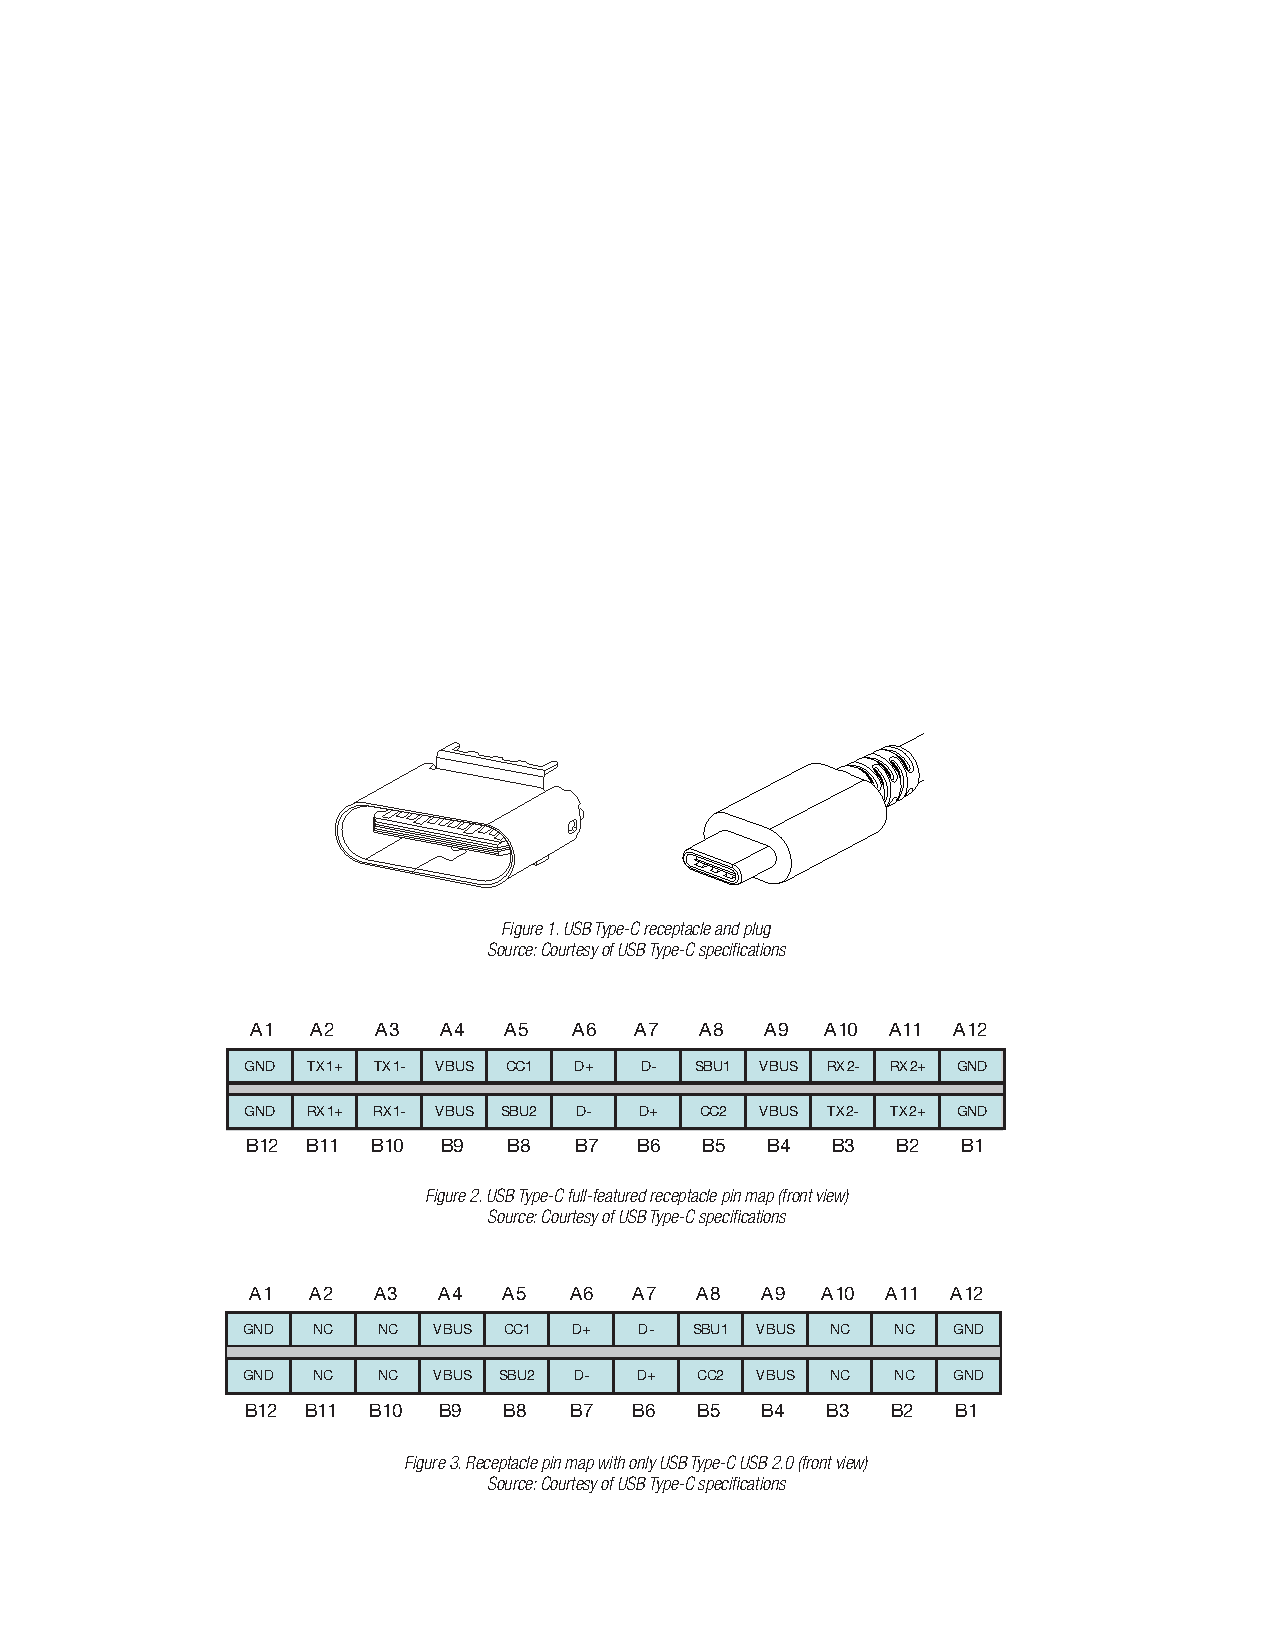
\includegraphics[width=\columnwidth]{USB-2-To-Type-C.pdf}
    \caption{USB-TypeC}
    \label{fig:USB-TypeC}
\end{figure}



\begin{figure}[htbp]
    \centering
    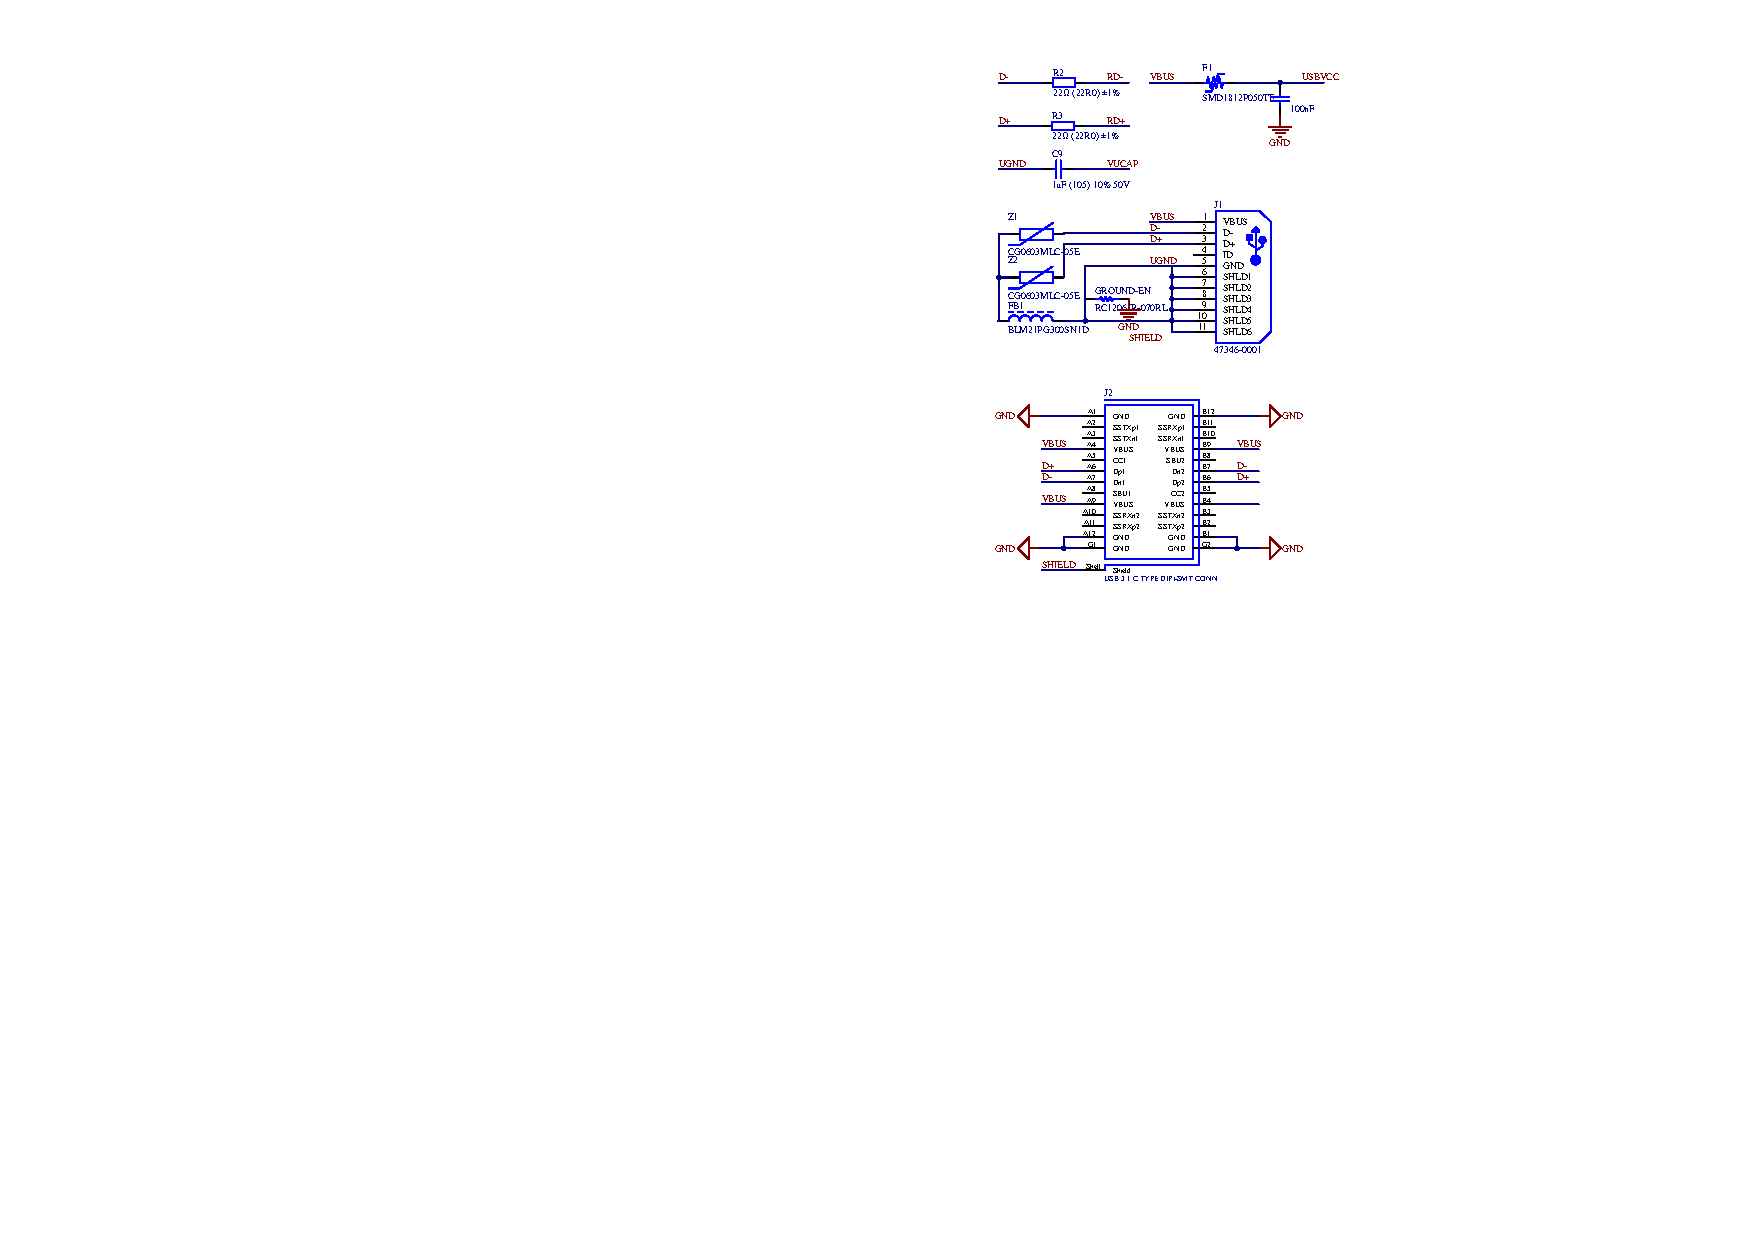
\includegraphics[]{Mega2560-USB.pdf}
    \caption{Mega2560-USB}
    \label{fig:Mega2560-USB}
\end{figure}

如图~\ref{fig:Mega2560-USB}:

BLM21PG300SN1D为(电感式)片式铁氧体磁珠,阻抗30Ω频率100MHz。

0603ESDA-05N为ESD抑制器/TVS二极管,箝位电压	50V,反向关断电压(典型值)	5V

USB口外壳和内部引线之间并联了ESD二极管和铁氧体磁珠,用于防USB浪涌电流,保护电路。

SMD1812P050TF为PTC自恢复保险丝,最大电压15V,保持电流500mA,最大电流100A,跳闸电流1A,为了防止USB输入电流持续过大。

USB 3.1 C TYPE DIP+SMT CONN为USB Type-C 母头,按照USB2.0协议使用,后续可添加PD或高速数据传输等功能。


\section{电机驱动}
之前使用的TB6612芯片近期国内断货,所以改用A4950、L293D等替代,但是没找到封装。

\section{RGBLED}

WS2812B是一个集控制电路与发光电路于一体的智能外控LED光源。其外型与一个5050LED灯珠相同,每个元件即为一个像素点。像素点内部包含了智能数字接口数据锁存信号整形放大驱动电路,还包含有高精度的内部振荡器和12V高压可编程定电流控制部分,有效保证了像素点光的颜色高度一致。

数据协议采用单线归零码的通讯方式,像素点在上电复位以后,DIN端接受从控制器传输过来的数据,首先送过来的24bit数据被第一个像素点提取后,送到像素点内部的数据锁存器,剩余的数据经过内部整形处理电路整形放大后通过DO端口开始转发输出给下一个级联的像素点,每经过一个像素点的传输,信号减少24bit。像素点采用自动整形转发技术,使得该像素点的级联个数不受信号传送的限制,仅仅受限信号传输速度要求。

LED具有低电压驱动,环保节能,亮度高,散射角度大,一致性好,超低功率,超长寿命等优点。将控制电路集成于LED上面,电路变得更加简单,体积小,安装更加简便。


\section{ESP32通信模块}

经过BLE4.2和ESP8266的原理性验证,选择ESP32作为通信模块和第二MCU使用。

Espressif ESP32 WROOM 系列\footnote{https://www.espressif.com/zh-hans/products/hardware/esp-wroom-32/overview},基于乐鑫先进的 SoC,ESP32 WROOM 系列模组具备高性能和丰富的外设,集成了 Wi-Fi和蓝牙功能,为先进的物联网应用提供了高度集成的解决方案。

ESP32 WROOM 系列模组包括 ESP32-WROOM-32,ESP32-WROOM-32D 和 ESP32-WROOM-32U 型号,集成了 ESP32 SoC,闪存,精密离散元件和 PCB 板载天线/IPEX 天线,该天线能够在空间有限的应用中提供出色射频性能。

ESP32 WROOM 系列模组具备优化的引脚布局,外设 IO 管脚被分组并引出,将外部走线降低,便于 PCB 板设计,从而使应用更加紧凑。

在本设计中,我们可以灵活选择使用ESP32-WROOM-32/32D/32DC模组,它们的封装和绝大多数功能完全一样。

\begin{figure}[htbp]
    \centering
    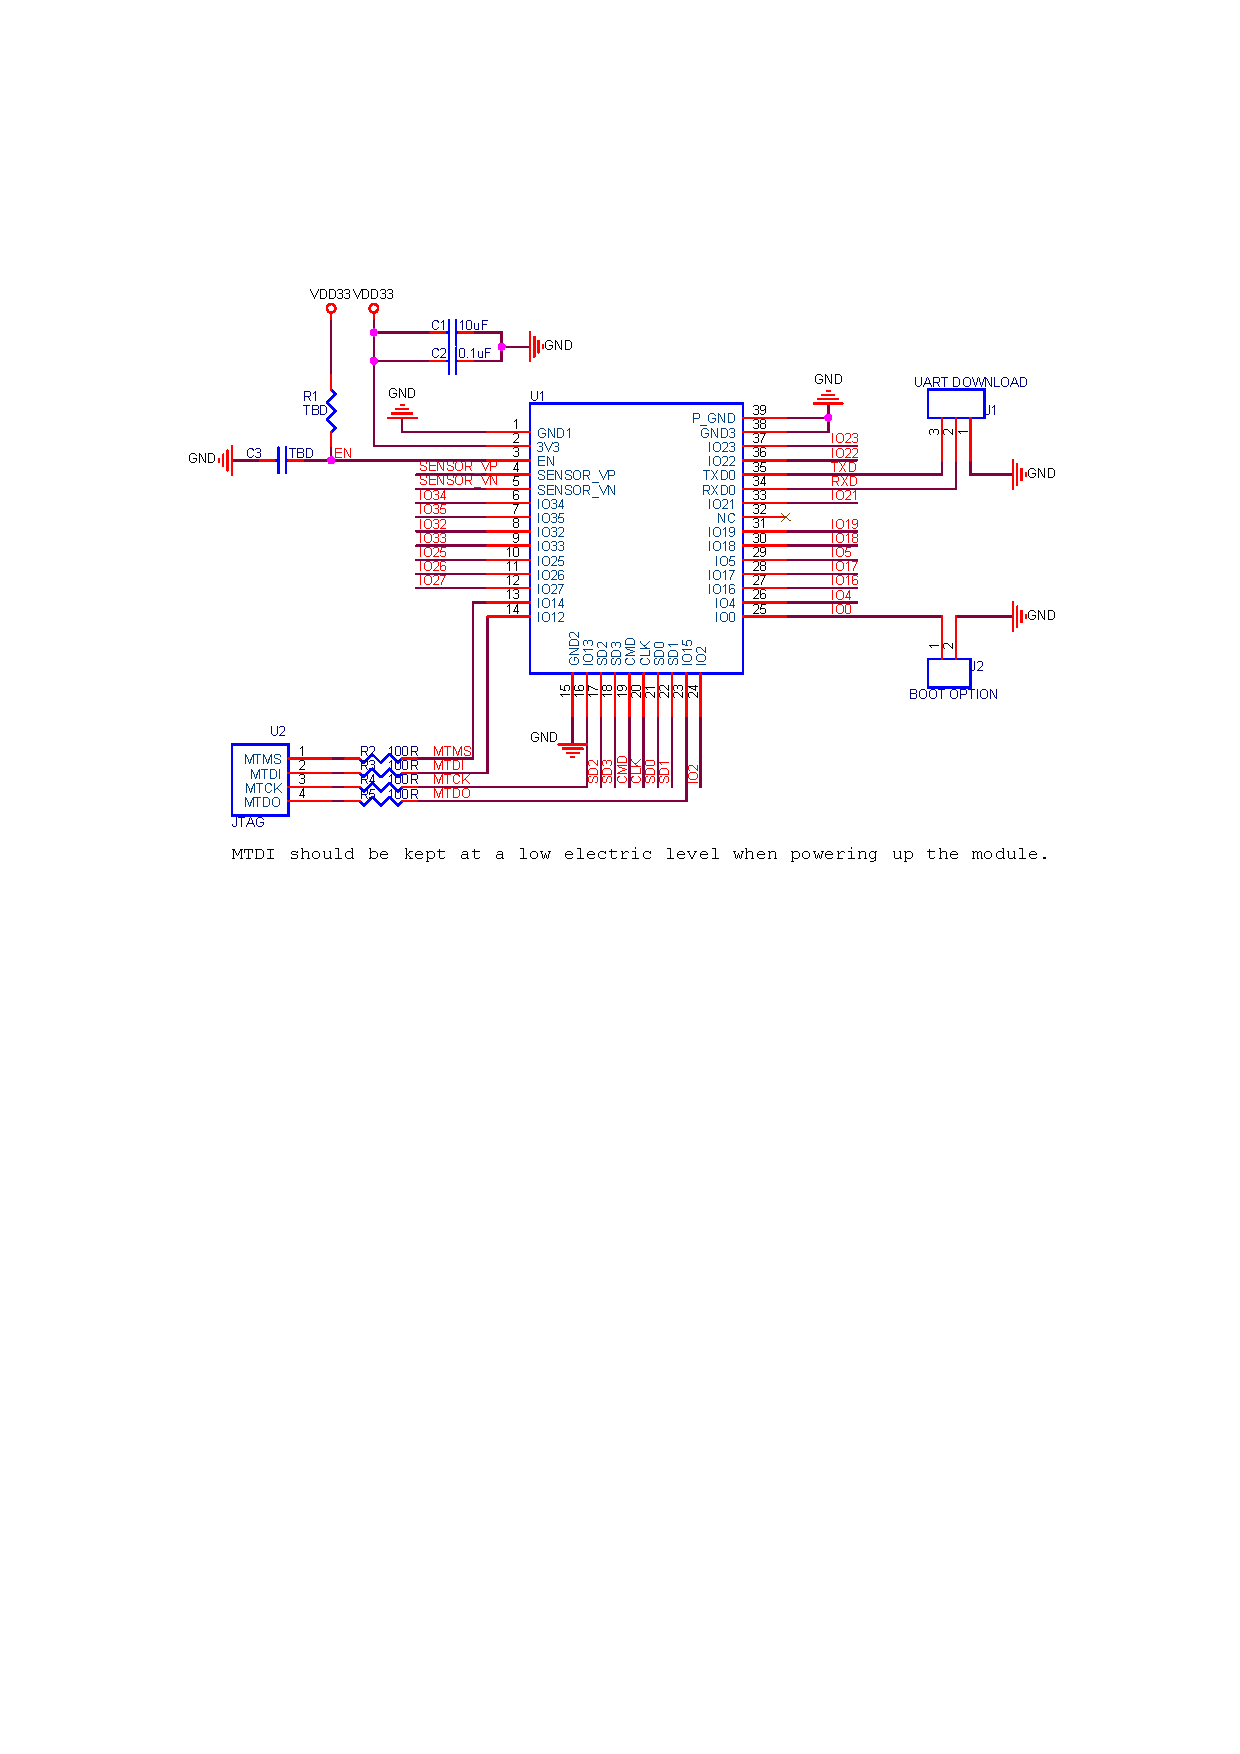
\includegraphics[width=\columnwidth]{esp32-wroom-32_datasheet_cn_Outside.pdf}
    \caption{ESP32-WROOM-32 外围原理图}
    \label{fig:ESP32Outside}
\end{figure}

如图~\ref{fig:ESP32Outside}:

注意:

\begin{itemize}
    \item MTDI 应保持低电平。
    \item ESP32-WROOM-32 管脚39,可以不焊接到底板。若将该管脚焊接到底板,确保使用适量的焊锡膏。
    \item 为确保芯片上电时的供电正常,EN管脚处需要增加RC延迟电路。RC通常建议为R = 10kOhms,C = 0.1uF,但具体数值仍需根据模组电源的上电时序和芯片的上电复位时序进行调整。
\end{itemize}

\begin{figure}[htbp]
    \centering
    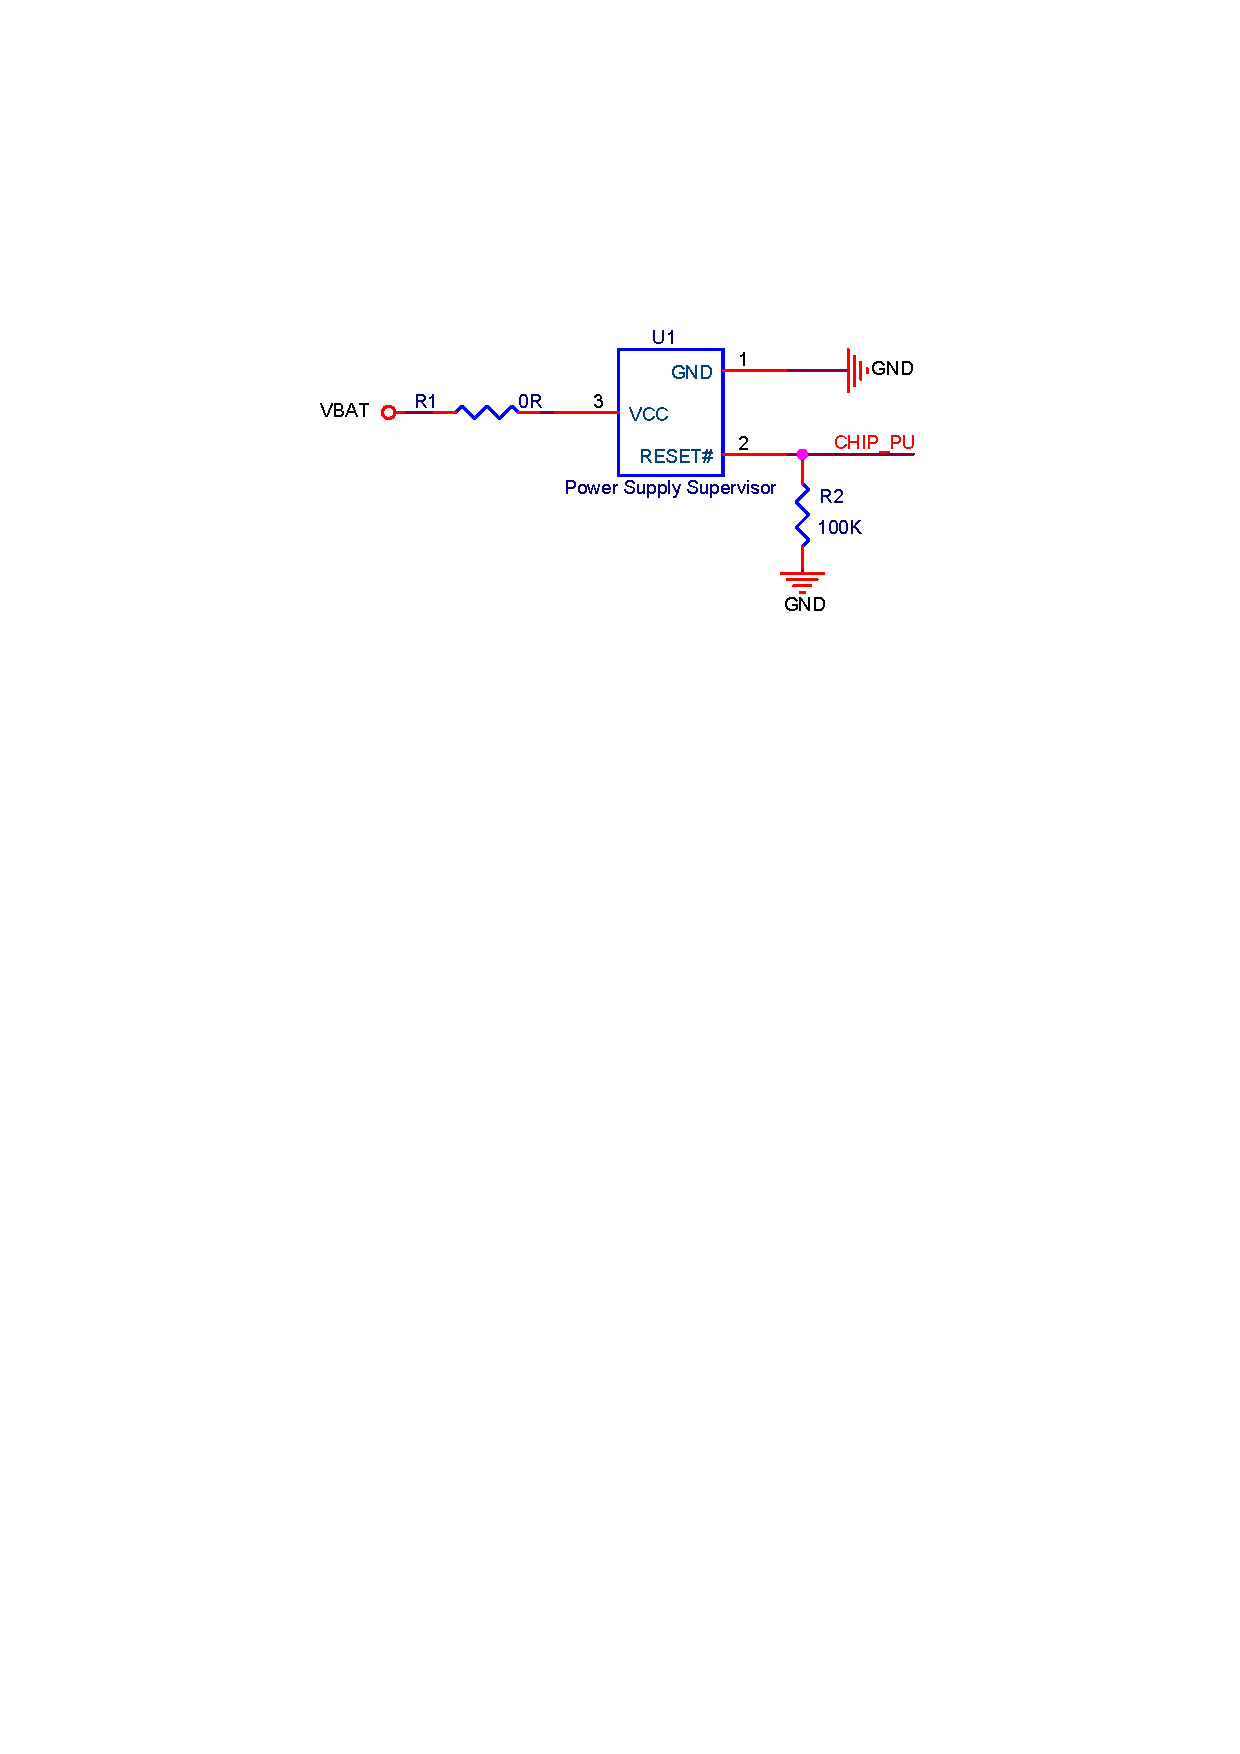
\includegraphics[]{esp32-wroom-32_datasheet_cn_Reset.pdf}
    \caption{ESP32-WROOM-32复位电路}
    \label{fig:ESP32Reset}
\end{figure}

如图~\ref{fig:ESP32Reset},当使用电池给ESP32系列芯片和模组供电时,为避免电池电压过低导致芯片进入异常状态不能正常启动,一般推荐外接Power Supply Supervisor。建议检测到供给ESP32的电压低于2.3V 时将ESP32的CHIP PU脚拉低。

% \begin{figure}
%     \begin{minipage}{0.48\textwidth}
%       \centering
%       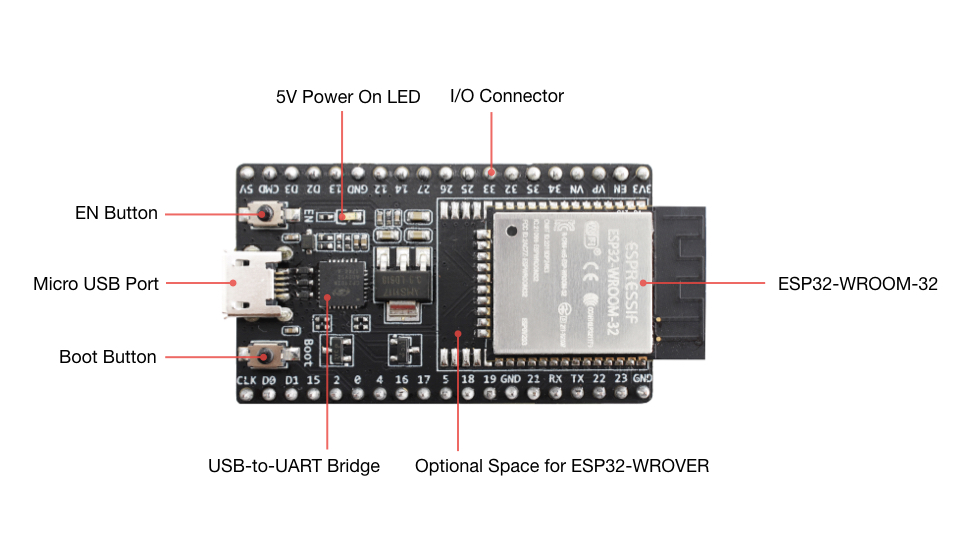
\includegraphics[width=\columnwidth]{ESP32-DevKitC-functional-overview.jpg}
%       \caption{ESP32-DevKitC实物图}
%       \label{fig:ESP32-1}
%     \end{minipage}\hfill
%     \begin{minipage}{0.48\textwidth}
%       \centering
%       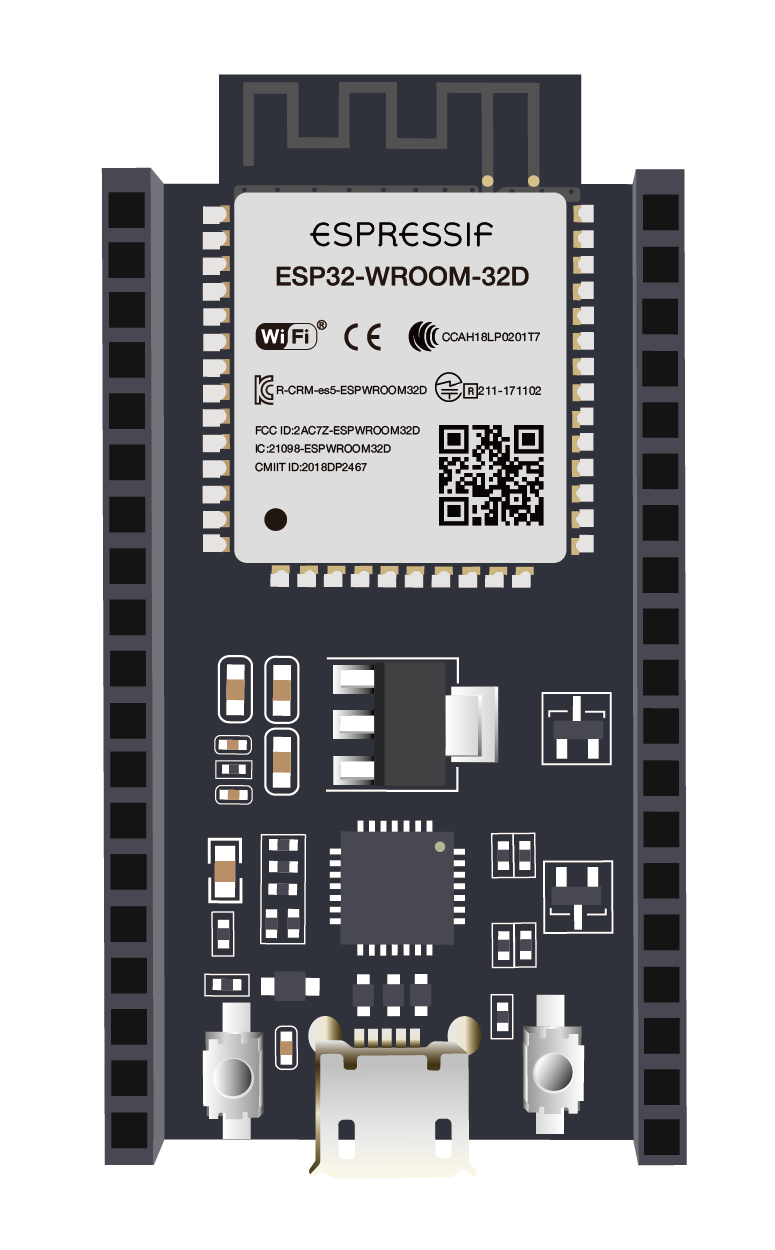
\includegraphics[width=\columnwidth]{ESP32-DevKitC-32D.png}
%       \caption{ESP32-DevKitC模型图}
%       \label{fig:ESP32-2}
%     \end{minipage}
% \end{figure}

\begin{figure}[htbp]
    \centering
    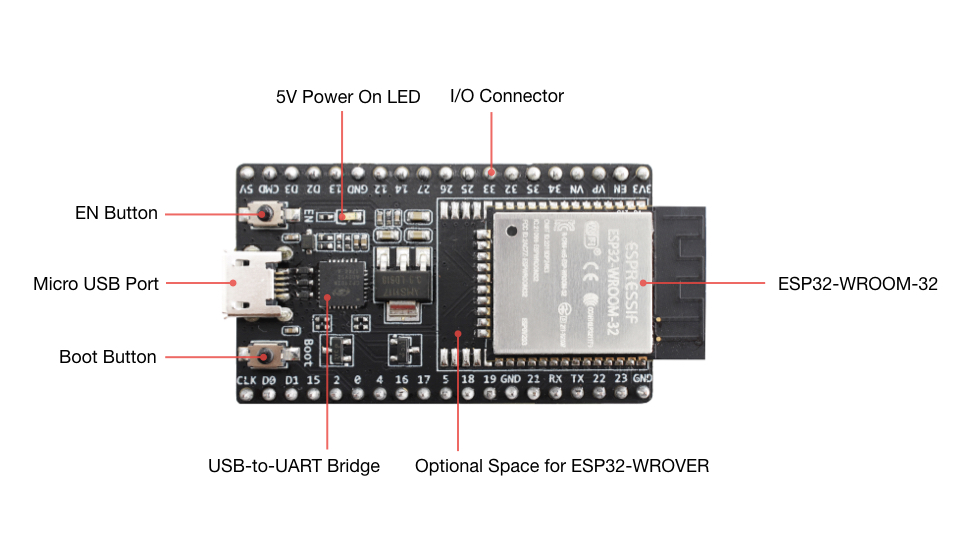
\includegraphics[width=\columnwidth]{ESP32-DevKitC-functional-overview.jpg}
    \caption{ESP32-DevKitC实物图}
    \label{fig:ESP32-1}
\end{figure}


\begin{figure}[htbp]
    \centering
    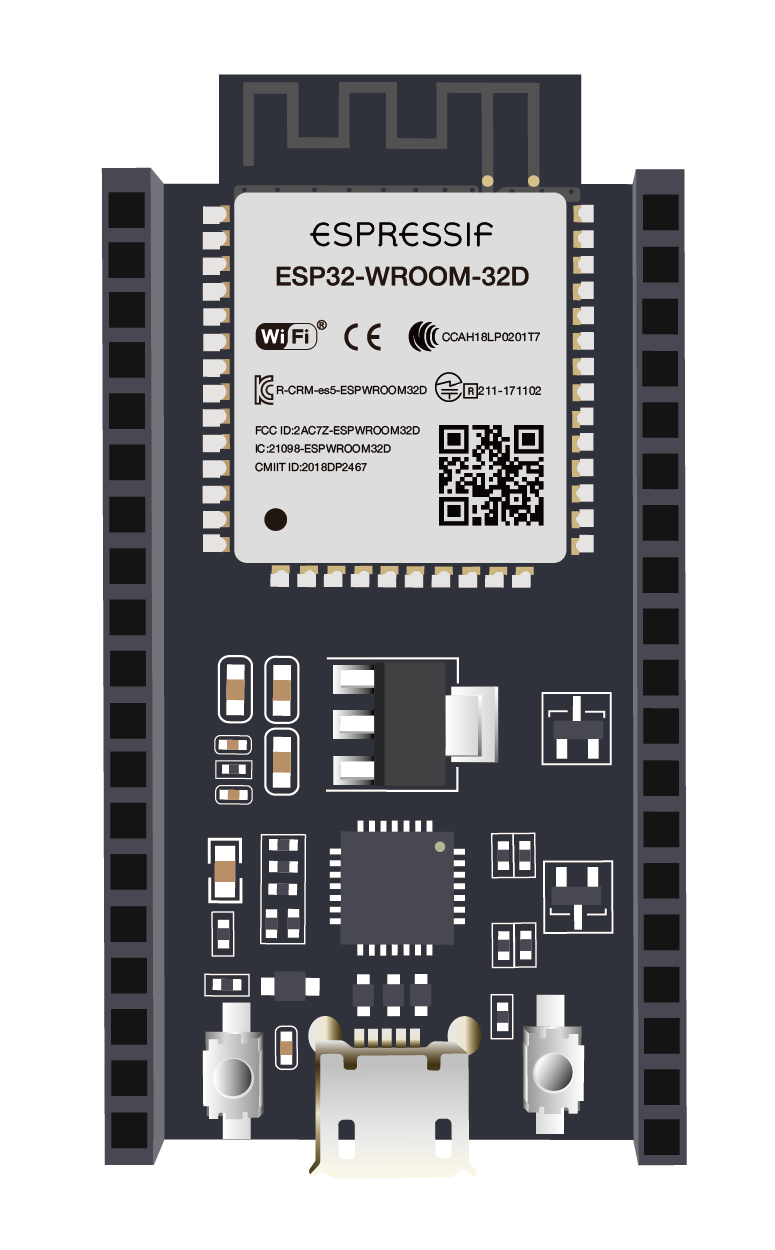
\includegraphics[width=0.48\textwidth]{ESP32-DevKitC-32D.png}
    \caption{ESP32-DevKitC模型图}
    \label{fig:ESP32-2}
\end{figure}

ESP32周边程序烧写设计参考ESP32-DevKitC V4\footnote{\url{https://docs.espressif.com/projects/esp-idf/zh_CN/latest/hw-reference/get-started-devkitc.html}}。如图~\ref{fig:ESP32-1},ESP32-DevKitC 是一款入门级开发板。板上集成的 ESP32 引脚均已引出,便于连接和使用。

管脚 D0、D1、D2、D3、CMD 和 CLK 用于 ESP32 芯片与 SPI flash 间的内部通信,集中分布在开发板两侧靠近 USB 端口的位置。通常而言,这些管脚最好不连,否则可能影响 SPI flash / SPI RAM 的工作。

管脚 GPIO16 和 GPIO17 仅适用于板载 ESP32-WROOM 系列和 ESP32-SOLO-1 的开发板,保留内部使用。

可以直接通过JTAG给ESP32烧写程序,可以通过UART烧写。

CP2102N-A01-GQFN20R作为USB-UART芯片,不使用其内置3.3V电压转换模块(即供电类型定义为自驱动而非USB总线驱动),通过此芯片可以直接通过USB给ESP32烧写程序。优点是廉价,缺点则为CP2102N只能烧写程序,而不能作为 USB-to-JTAG 接口进行ESP32和计算机的实时通信桥梁。

\begin{figure}[htbp]
    \centering
    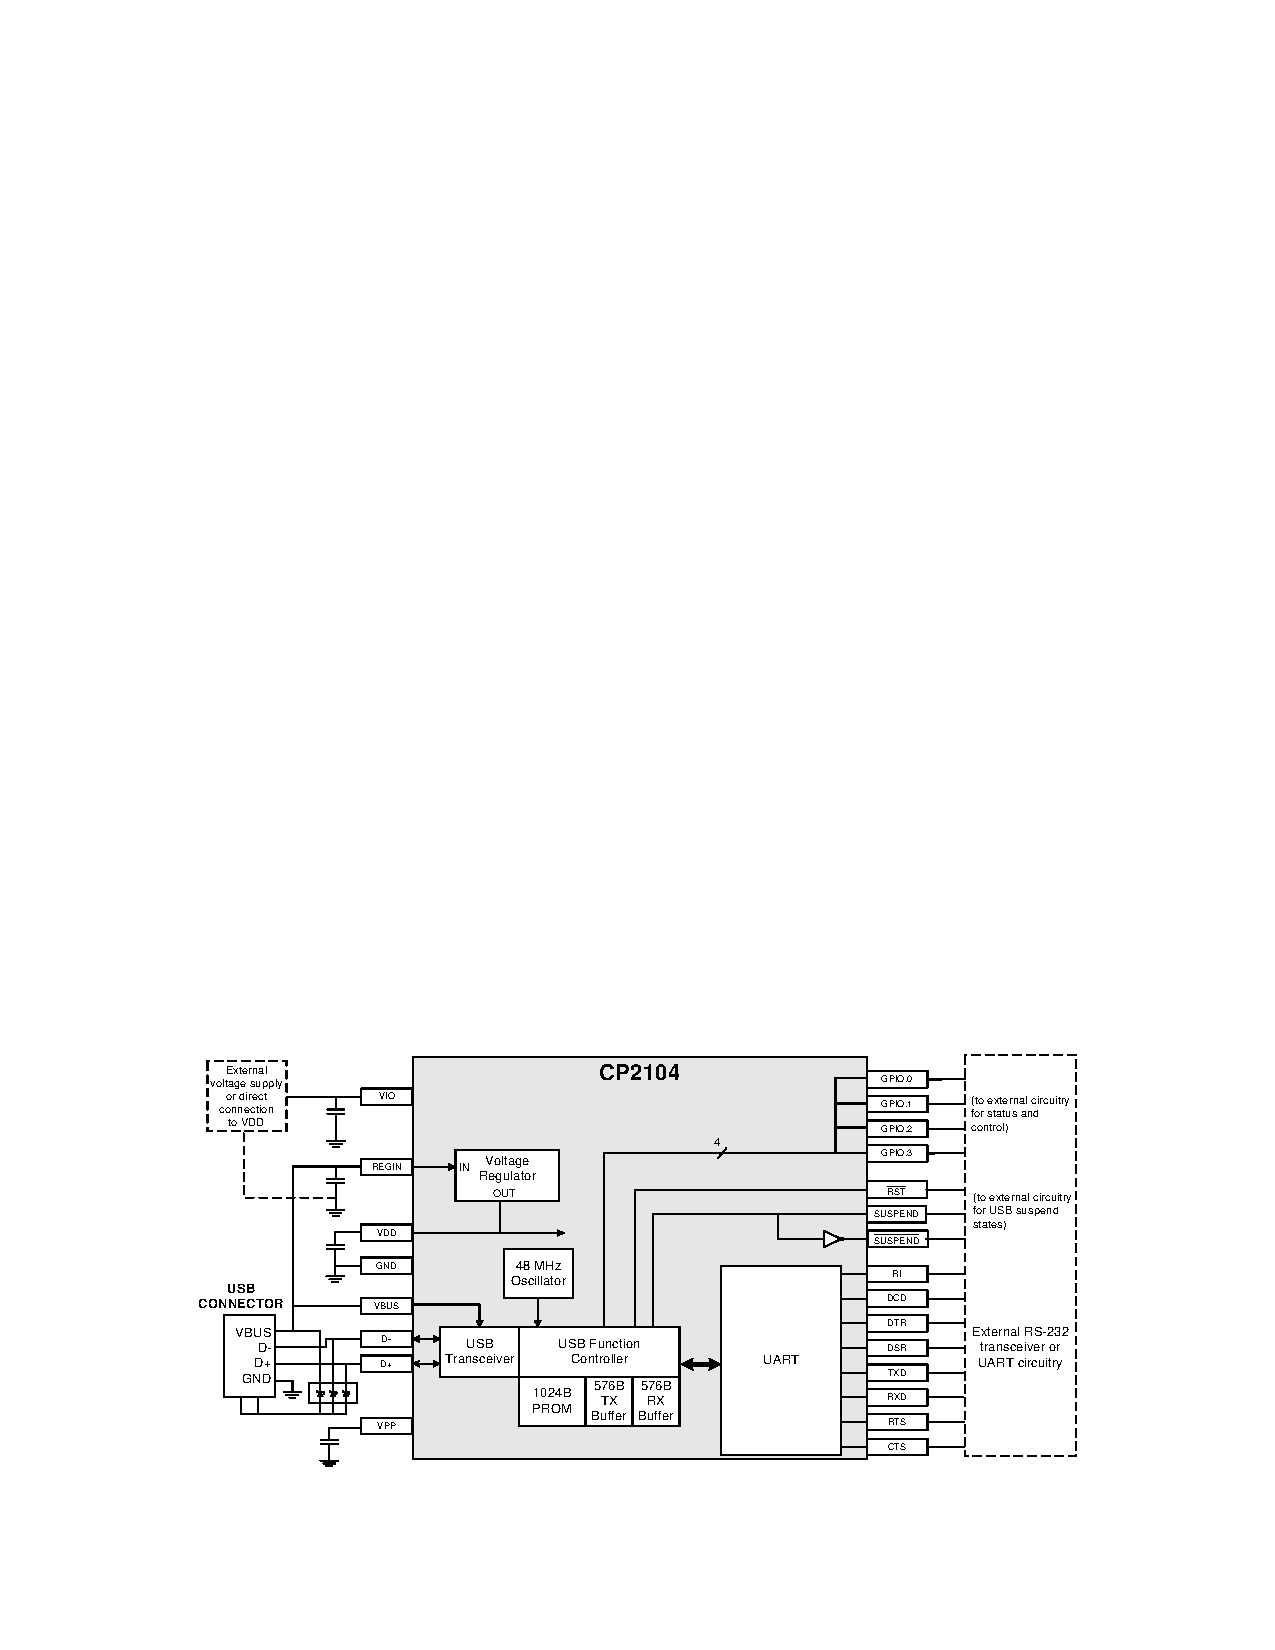
\includegraphics[]{CP2104-F03-GMR_System.pdf}
    \caption{CP2104-F03-GMR系统示例图}
    \label{fig:CP2104-F03-GMR}
\end{figure}

后更新为QFN-24-4x4x05P封装的CP2104-F03-GMR芯片,如图~\ref{fig:CP2104-F03-GMR},这一版本的设计参考了官方Datasheet和Github开源项目ESP-Debugger\footnote{\url{https://github.com/xiongyumail/ESP-Debugger}}中的部分电路。

\begin{figure}[htbp]
    \centering
    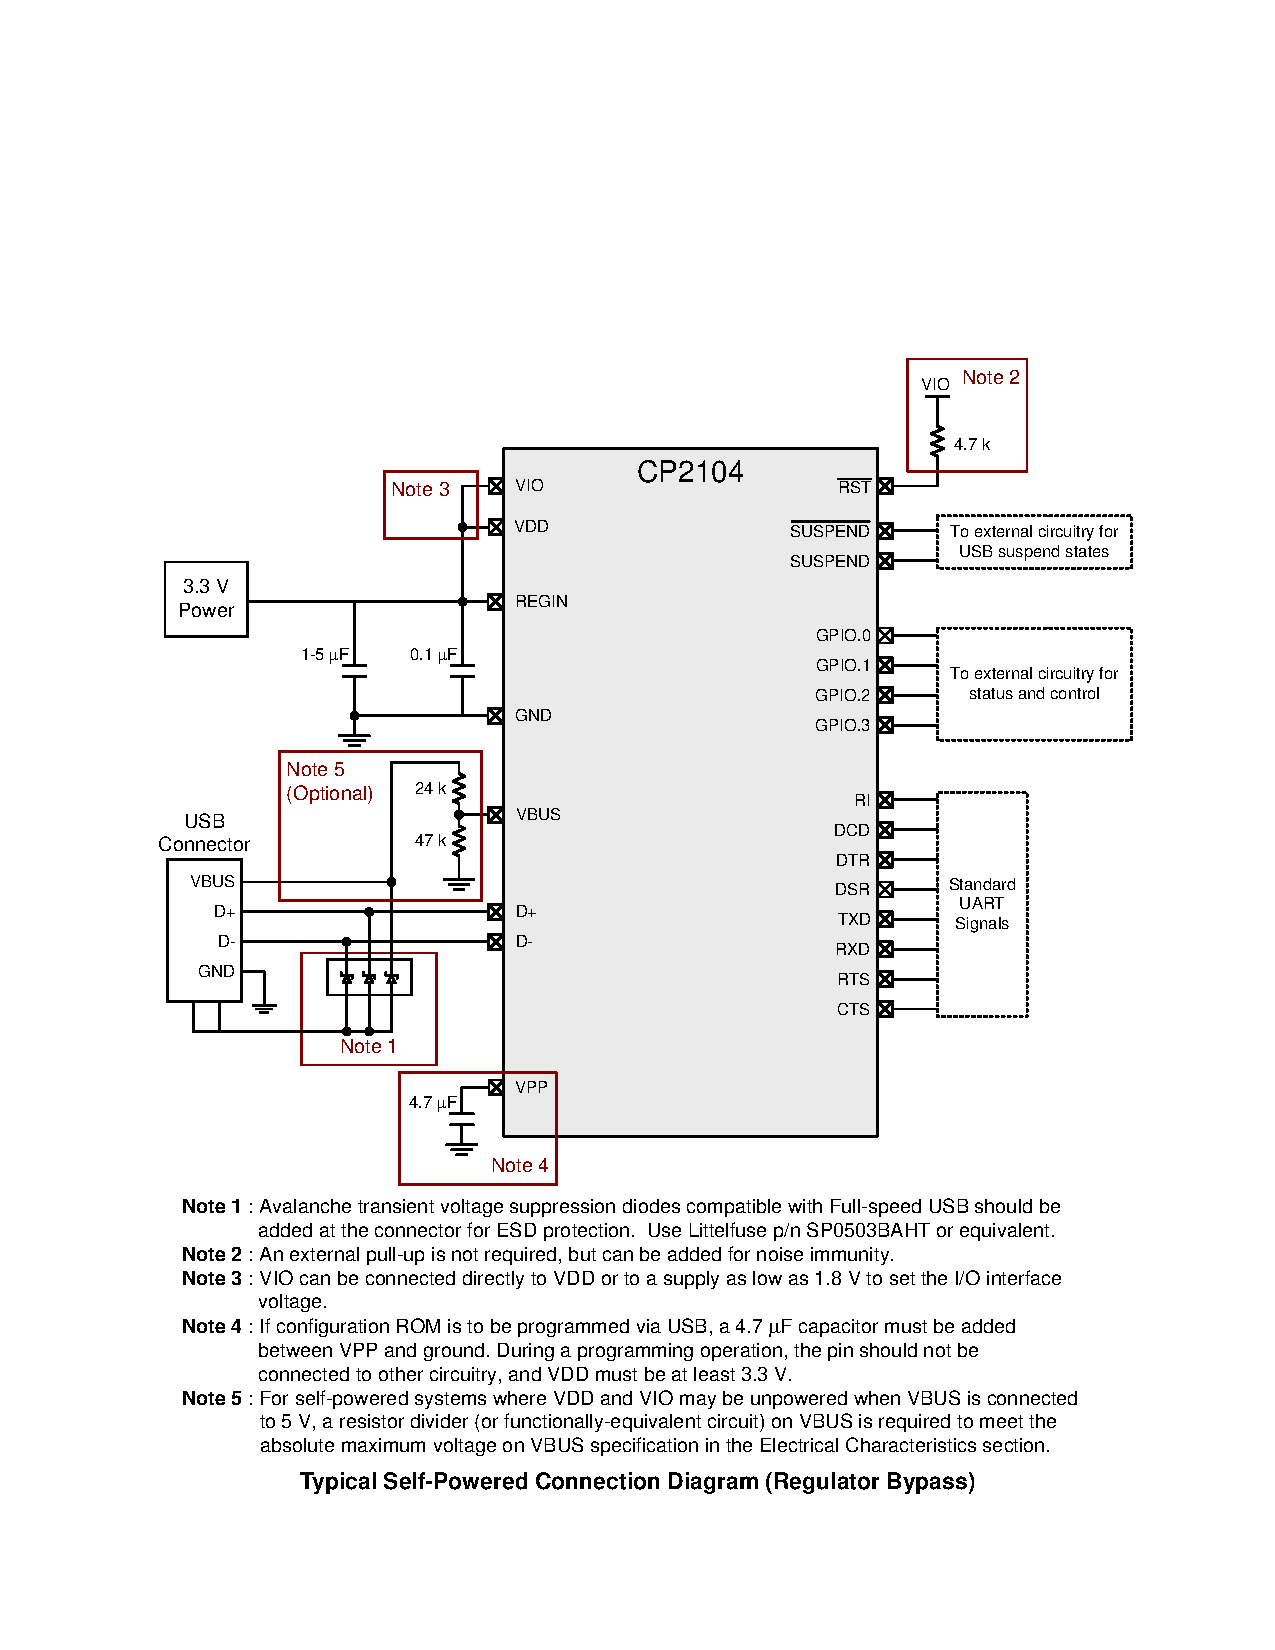
\includegraphics[]{CP2104-F03-GMR-Regulator-Bypass.pdf}
    \caption{CP2104不使用电平转换示例图}
    \label{fig:CP2104-Regulator-Bypass}
\end{figure}

如图~\ref{fig:CP2104-Regulator-Bypass},在本项目中,VIO和VDD连在一起并通过4.7kOhm的电阻和RST连在一起,REGIN也和VIO VDD连起来,靠近这三个引脚的地方有1uF和100nF的接地电容滤波。另外,接入芯片VBUS的是USB输入的5V经过电阻分压得到的接近3.3V的电压。


% \begin{figure}[htbp]
%     \centering
%     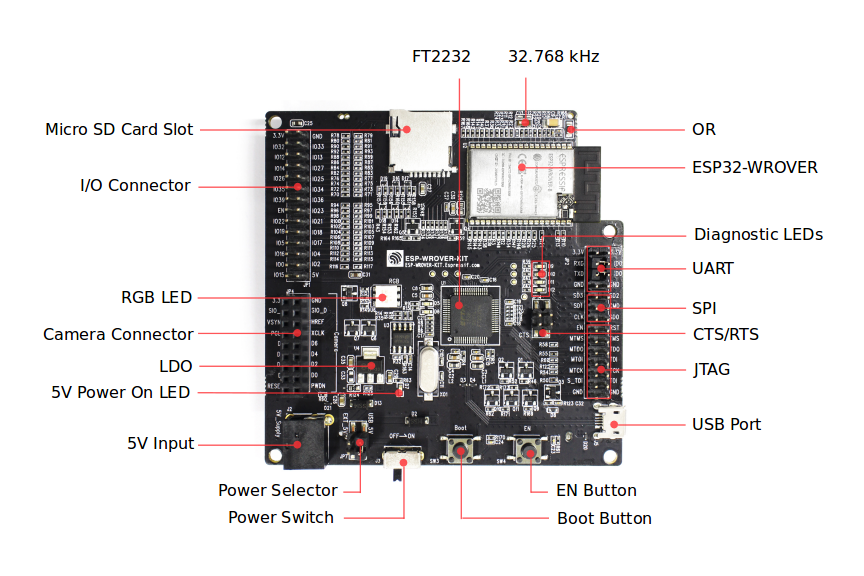
\includegraphics[]{esp-wrover-kit-v4.1-layout-front.png}
%     \caption{ESP WROVER KIT实物图}
%     \label{fig:ESP32-WROVER-0}
% \end{figure}

\begin{figure}[htbp]
    \centering
    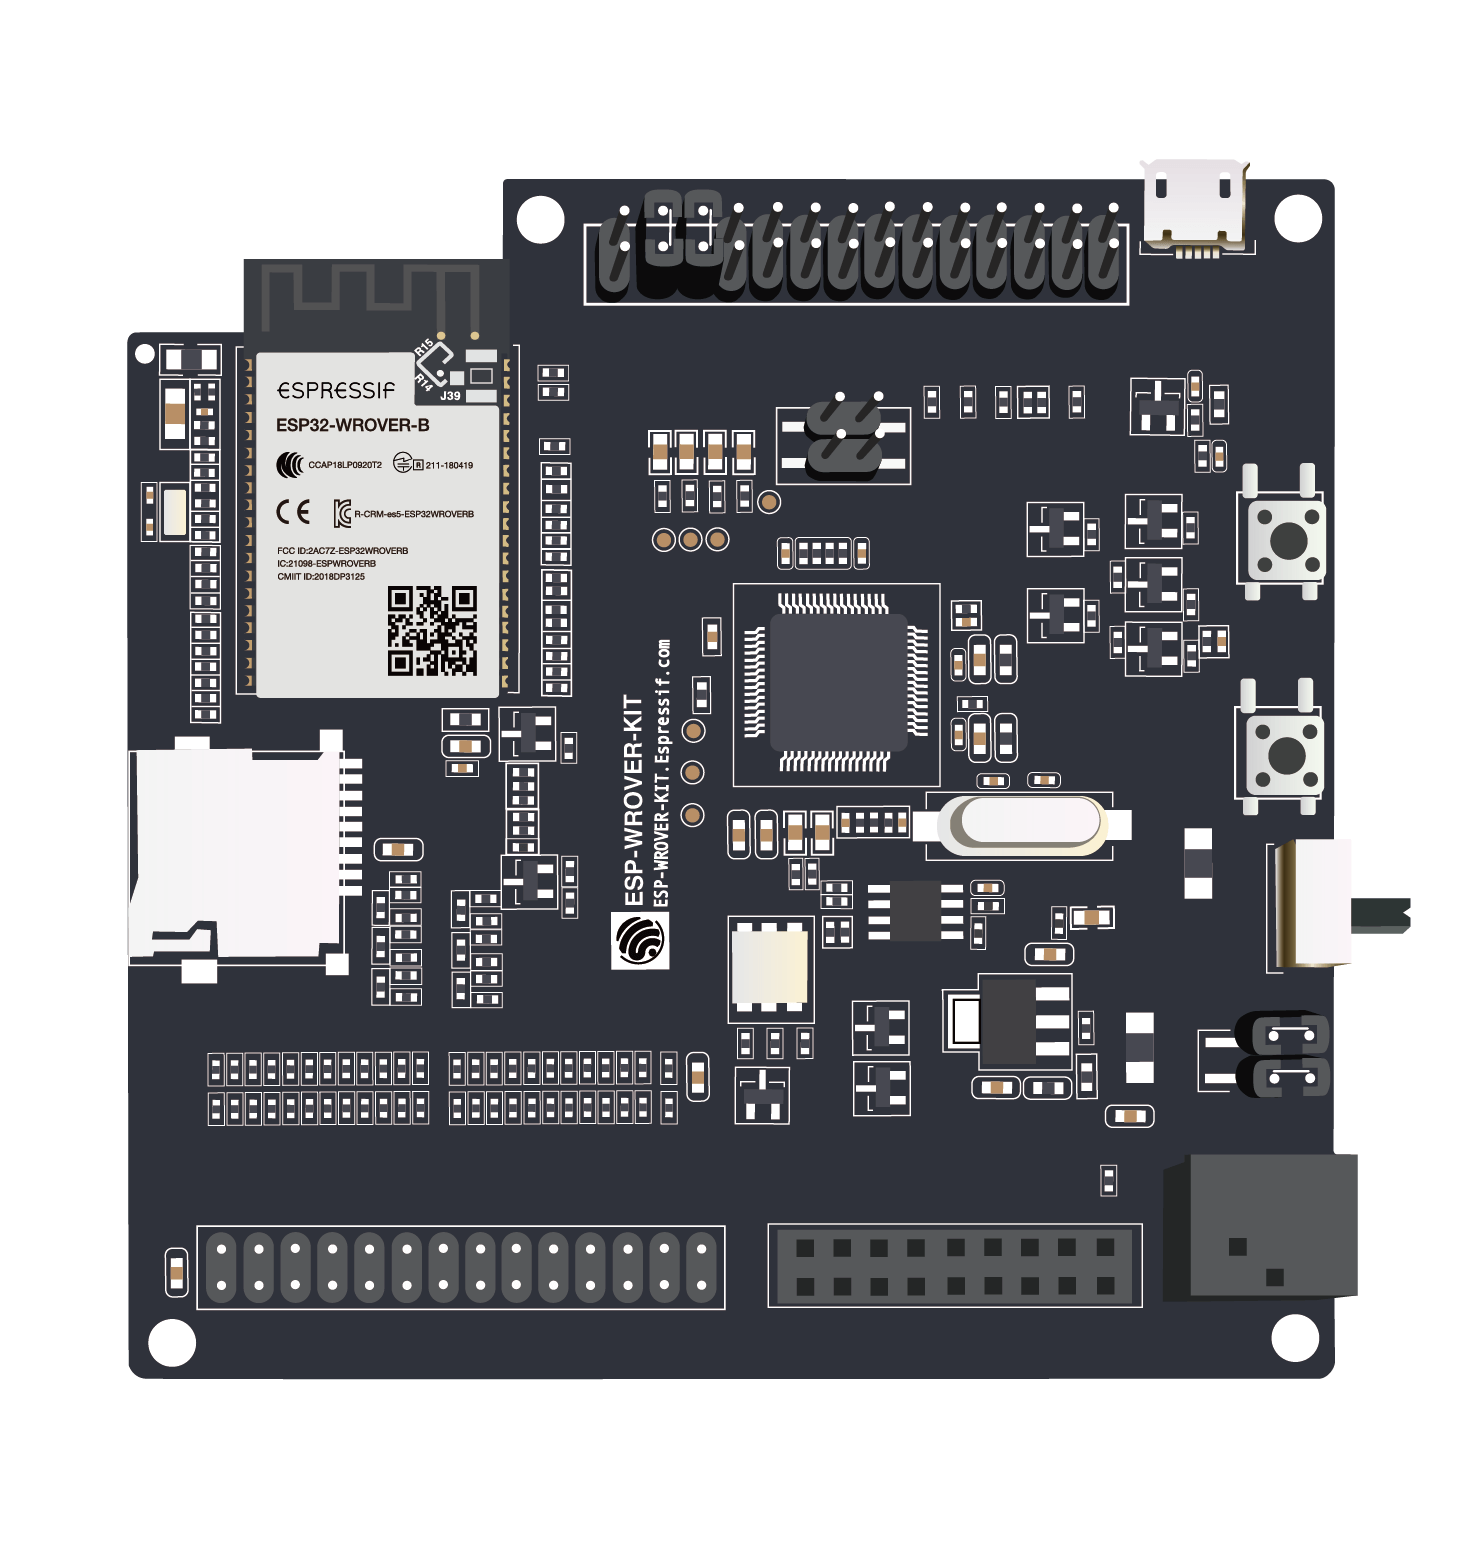
\includegraphics[width=0.7\columnwidth]{esp-wrover-kit-vb.png}
    \caption{ESP WROVER KIT模型图}
    \label{fig:ESP32-WROVER}
\end{figure}

参考ESP WROVER KIT(如图~\ref{fig:ESP32-WROVER})设计。ESP-WROVER-KIT-VB 为乐鑫 ESP-WROVER-KIT 开发板的变体,默认贴片 ESP32-WROVER-B 模组,支持 LCD 和 MircoSD 卡。板上 ESP32-WROVER-B 模组的 I/O 管脚均已引出,允许用户连接丰富的外设,满足多种开发场景。此外,本款开发板还载有支持多种协议的 USB 转接桥 (FTDI FT2232HL),允许用户直接通过 USB 接口使用 JTAG 调试 ESP32 模组,极大地降低了二次开发的复杂度和成本。

FT2232 多协议 USB 转串口桥接器。开发人员可通过 USB 接口对 FT2232 芯片进行控制和编程,与 ESP32 建立连接。FT2232 芯片可在通道 A 提供 USB-to-JTAG 接口功能,并在通道 B 提供 USB-to-Serial 接口功能,便利开发人员的应用开发与调试。详见 ESP-WROVER-KIT V4.1 原理图。



\section{扩展接口}

三明治扩展形式,层层堆叠。

